\documentclass[reprint, superscriptaddress, floatfix]{revtex4-1}
\usepackage{amsmath}
\usepackage{amsfonts}
\usepackage{mathtools}
\usepackage{upgreek}
\usepackage[table,usenames,dvipsnames]{xcolor}
\usepackage{tikz}
\usetikzlibrary{calc}
\usepackage{hyperref}
\usepackage{setspace}

\hypersetup{
  colorlinks,
  linkcolor={red!30!black},
  citecolor={green!20!black},
  urlcolor={blue!80!black}
}


\definecolor{DarkBlue}{RGB}{0,0,64}
\definecolor{DarkBrown}{RGB}{64,20,10}
\definecolor{DarkGreen}{RGB}{0,64,0}
\definecolor{DarkPurple}{RGB}{64,0,42}
\definecolor{LightGray}{gray}{0.85}
% annotation macros
\newcommand{\repl}[2]{{\color{gray} [#1] }{\color{blue} #2}}
\newcommand{\add}[1]{{\color{blue} #1}}
\newcommand{\del}[1]{{\color{gray} [#1]}}
\newcommand{\note}[1]{{\color{DarkGreen}\footnotesize \textsc{Note.} #1}}
\newcommand{\answer}[1]{{\color{DarkBlue}\footnotesize \textsc{Answer.} #1}}
\newcommand{\summary}[1]{{\color{DarkPurple}\footnotesize \textsc{Summary.} #1}}


\newcommand{\Err}{E}
\newcommand{\ii}{\mathrm{i}}
%bin average
\newcommand{\bav}[1]{#1_\mathrm{av}}


\begin{document}



\title{Optimal updating factor in adaptive flat-distribution-sampling simulations}

\author{Cheng Zhang}
\author{Justin A. Drake}
\affiliation{
Sealy Center for Structural Biology and Molecular Biophysics,
The University of Texas Medical Branch,
Galveston, Texas 77555-0304, USA}
\author{Jianpeng Ma}
\affiliation{
Department of Biochemistry and Molecular Biology,
Baylor College of Medicine, Houston, Texas 77030, USA}
\affiliation{
Department of Bioengineering,
Rice University, Houston, Texas 77005, USA}
\author{B. Montgomery Pettitt}
\email{bmpettitt@utmb.edu}
\affiliation{
Sealy Center for Structural Biology and Molecular Biophysics,
The University of Texas Medical Branch,
Galveston, Texas 77555-0304, USA}



\begin{abstract}
  We present a method of computing the optimal schedule
  of the updating magnitude
  for a class of flat-distribution sampling methods
  for free energy calculation including
  the Wang-Landau (WL) algorithm and metadynamics.
  %
  These methods rely on adaptive construction of
  a bias potential that offsets
  the potential of mean force by histogram-based adaptive updates.
  %
  The updating magnitude should decrease over time
  to reduce the error in the bias potential,
  and one may speed up the convergence by choosing an optimal schedule
  of the updating magnitude.
  %
  %Here, we will show that the optimal schedule
  %can be derived
  %from a mechanical analogy, in which
  %the schedule corresponds to
  %the velocity of a free particle with a position-dependent mass
  %and the final error serves as the action.
  %%
  %Therefore, the optimal schedule follows from
  %the equation of motion of the particle.
  %
  We will show that
  the optimal schedule depends on the updating scheme.
  %
  While the asymptotically optimal schedule for
  the single-bin updating scheme (commonly used in WL)
  is given by inverse-time formula,
  that for the Gaussian updating scheme (commonly used in metadynamics)
  is often more complex.
  %and the initial updating magnitude is ideally half of
  %the previous equilibrium value.
  %
  Further,
  we show that the single-bin updating scheme
  belongs to a class of bandpass updating schemes
  that are optimal for asymptotic convergence.
  %
  These bandpass updating schemes aim at
  partially flattening a few selected histogram modes
  and their optimal schedule
  is also given by the inverse-time prescription.
  %
  Several previous flat-distribution-sampling algorithms
  can be cast as special cases of the bandpass updating schemes.
  %
\end{abstract}

\maketitle



\section{Introduction}



Free energy calculation\cite{frenkel, newman} is a central theme
in computational physics and chemistry
that can provide insight into an array of phenomena not easily studied
with traditional experiments.
%
Given a system,
often the task is to compute
a distribution, $p^*(z)$,
along a collective variable, $z$, by sampling via either Monte Carlo\cite{
  frenkel, newman, landau_binder} (MC)
or molecular dynamics\cite{frenkel, karplus2002} (MD) simulations.
%
The dimensionless free energy, or potential of mean force (PMF),
along the collective variable, $z$,
is $-\ln p^*(z)$.
%
However, accurately estimating the PMF is often difficult
when the collective variable is energetically restricted to local regions
of the complex, multimodal free energy surface.
%
Thus,
to overcome these energetic barriers and
to capture the global shape of the free energy surface
an effective strategy is to introduce a bias potential that
cancels the PMF.
%
Ideally, then, sampling yields a flat distribution
along $z$\cite{mezei1987, berg1992, *lee1993,
wang2001, *wang2001pre,
huber1994,
*laio2002, *laio2008, *barducci2011, *sutto2012}.
%
The flat-distribution sampling can be used to accelerate
sampling of slow transitions that otherwise would not readily
be observed with traditional simulations.
%
%A better solution is to artificially flatten
%the target distribution along $z$\cite{mezei1987, berg1992, *lee1993,
%wang2001, *wang2001pre,
%huber1994,
%*laio2002, *laio2008, *barducci2011, *sutto2012}.
%%
%This alleviates the above problem of local trapping
%by forcing the system to travel more
%deliberately along $z$,
%which often represents
%a direction of slow motion.
%%
%To achieve a flat distribution, however,
%the method must be able to construct a
%bias potential that cancels the PMF.



Many efficient flat-distribution-sampling (FDS) techniques
based on adaptive construction of the bias potential
have been introduced,
including the Wang-Landau (WL) algorithm\cite{
  wang2001, *wang2001pre}
and metadynamics\cite{huber1994,
*laio2002, *laio2008, *barducci2011, *sutto2012},
popular for MC and MD simulations, respectively\cite{junghans2014}.
%
%flat-distribution-sampling (FDS) techniques
%that build the bias potential adaptively or on the fly.
%
These techniques regularly update the bias potential
to discourage future visits to previously sampled configurations
by incrementally elevating the bias potential,
%and they are closely-related\cite{junghans2014, micheletti2004}.
%
%The bias potential is associated with discrete values of $z$.
%
A key difference lies
in the updating window function,
which specifies
a neighborhood around the current value of
$z$ on the free energy surface
where the updating should occur
as well as the relative updating magnitude.
%
Usually, the window function
takes the form of a discrete
$\delta$-function (a boxcar function one histogram bin wide)
in WL,
or that of a Gaussian
in metadynamics.
%
Although the two window functions
are not always associated with
the two methods\cite{micheletti2004, kim2006, *kim2007, junghans2014},
we will colloquially use the terms WL and metadynamics
to represent FDS simulations using the
single-bin and Gaussian window functions, respectively.
%
%is that in the WL case,
%each updating step is limited to the bin
%containing the current $z$,
%while metadynamics adopts an extended
%Gaussian window
%covering several neighboring bins.
%%
%The latter is more often used in MD simulations
%as it guarantees a smooth profile
%of the bias potential
%suitable for numerical differentiation
%in deriving the bias force.
%
In both cases,
regular updates to the bias potential
%in both cases, the bias potential
%is updated frequently (usually every few MC or MD steps),
%and the fluctuation
disrupts the underlying equilibrium
sampling\cite{zhou2005, morozov2007, zhou2008},
and for convergence of the estimated PMF
one  has to gradually decrease
the updating magnitude of the bias.



The schedule of reducing
the updating magnitude,
therefore, critically affects
the precision of the final bias potential,
and hence that of the PMF\cite{laio2005, bussi2006, poulain2006,
belardinelli2007, *belardinelli2007jcp, *belardinelli2008, *belardinelli2016,
liang2007, min2007,
morozov2007, zhou2008,
komura2012, *caparica2012, *caparica2014,
barducci2008, dickson2011, dama2014}.
%
For the single-bin case, the optimal updating schedule
is a function of the
inverse time\cite{
belardinelli2007, *belardinelli2007jcp, *belardinelli2008, *belardinelli2016,
liang2007,
morozov2007, zhou2008}
or
the inverse number of updating steps.
\note{
  About the origin of the inverse-time formula.
  Besides the Belardinelli paper,
  we can also find it in Eq. (6) of reference \cite{liang2007},
  if I am not too mistaken.
  But I find the paper is a bit hard to read.
  There, however, the formula is $t_0/t$ instead of $1/t$.
}
The same schedule also applies to a variant of
the WL algorithm\cite{langfeld2012, pellegrini2014}.
%
%The optimal schedule for metadynamics,
%however, is less studied.


In this study,
we present a method of computing
the optimal schedule
for an adaptive FDS method
of a general updating scheme,
including the single-bin and Gaussian one
used in the WL algorithm and metadynamics.
%
Our method maps the optimization problem to a mechanical one,
in which the schedule plays the role of the velocity of
a free particle with a position-dependent mass,
and the final error becomes the action.
%
In this way, the optimal schedule
can be deduced from the equation of motion
of the particle that minimizes the action.
%
The resulting optimal schedule
depends on the updating window function
through the mass function.
%
While the optimal schedule in the single-bin case
is given by the known inverse-time formula,
that for Gaussian case is more complex
and sensitive to the simulation length
and the width of the Gaussian window.
%
%In either case, however,
%Ideally,
%the optimal initial updating magnitude
%can be set to
%half of the previous equilibrium value,
%which amounts to a shift of the origin of time
%in the single-bin case.
%
Further, we will show that
the single-bin updating scheme
is optimal for asymptotic convergence,
and it can be generalized
to a class of asymptotically optimal
bandpass updating schemes.
%
The latter, however,
allow one to selectively flatten only
a few long-range histogram modes,
and to avoid introducing local noise
into the bias potential during the updating process.
%
The optimal schedule of bandpass updating schemes
is also the above origin-shifted inverse-time schedule.
%
Interestingly, several previous FDS algorithms\cite{
  langfeld2012, pellegrini2014,
  neuhaus2006, *neuhaus2007}
can be cast as special cases of bandpass updating schemes.

%For finite-length simulations, however,
%metadynamics may deliver better performance.
%
%These results may help to better
%plan and optimize FDS simulations.



The article is organized as follows.
%
We present the analytical results in Sec. \ref{sec:theory},
numerically verify some aspects
in Sec. \ref{sec:results},
and conclude the article
in Sec. \ref{sec:conclusion}.




\section{\label{sec:theory}
Theory}



We develop the theory
in the following order.
%
In Sec. \ref{sec:background},
we first review the basics of FDS
and some known aspects of the optimal schedule.
%
Then, in Sec. \ref{sec:single-bin},
we illustrate the method of
computing the optimal schedule
in the simple case of the
single-bin updating scheme
used by the WL algorithm,
by proving the optimality
of the known inverse-time formula.
%
The above two introductory sections help define our notations,
and an expert reader may wish to skip them.
%
Next, we extend the method to the general case
of a multiple-bin updating scheme
that encompasses the Gaussian scheme used in metadynamics
in Sec. \ref{sec:multiple-bin},
and present a general procedure of computing the optimal schedule
in Sec. \ref{sec:procedure}.
%
Finally, we compare different updating schemes
and show that the single-bin scheme
and a class of generalized bandpass schemes
are optimal for convergence
in the long time or extensive sampling limit
in Sec. \ref{sec:cmpschemes}.



\subsection{\label{sec:background}
Background}



\subsubsection{\label{sec:FDS}
Flat-distribution sampling}



Consider the problem of computing
the distribution, $p^*_i$,
along a discrete quantity, $i$,
for a given system.
%
%For example, $i$ can be the energy, $E$,
%in a lattice spin model or the temperature index
%in a simulated tempering simulation\cite{
%marinari1992, *lyubartsev1992}.
%
For a continuous quantity, $z$,
%which is often the case in a (classical) molecular system,
we can discretize it
such that the integer $i$ represents
the index of a small interval, or a bin,
$(z, z + \Delta z)$.
%
%The distribution is normalized as
%$\sum_{i = 1}^n p^*_i = 1$.



%For a large system at temperatures of interest,
%the distribution, $p^*_i$, often tends to
%be localized,
%%
%and to explore the global shape
%of the PMF, $-\ln p^*_i$,
%it is often advantageous to perform
%biased sampling that targets
%a wider and smoother distribution, $p_i$.
%%
%%Here, we refer to simulations that target
%%a flat or nearly flat distribution
%%as entropic or multicanonical sampling.
%
%To do so, we introduce a bias potential, $u_i$,
The challenge of sampling a multimodal distribution, $p^*_i$,
with deep valley(s) can often be eased by
biased sampling targeting a smoother distribution, $p_i$.
%
%
%where the proportionality constant, $C_i$,
%is found from the normalization condition,
%$\sum_{i = 1}^n \pi_i = 1$,
%in the second step.
%
%In particular,
%to make $\pi_i$ flat,
%the bias potential $u_i$
%must coincide with $\ln p^*_i$,
%up to an additive constant.
%%
%In practice, $u_i$ may be non-optimal or contain error,
%and thus $\pi_i$ need not
%coincide with the intended distribution $p_i$.
%
We will broadly define
a flat-distribution-sampling (FDS) simulation
as a biased simulation
targeting a flat $p_i$ (i.e. $p_i \equiv 1/n$)
or nearly flat one\cite{
dayal2004, *trebst2004, barducci2008, singh2011}.
%
By introducing a bias potential, $u_i$,
the biased equilibrium distribution becomes
%
\begin{equation}
  \pi_i
  %=
  %C_i \, p^*_i \, e^{-u_i}
  =
  \frac{                p^*_i \, e^{-u_i} }
       { \sum_{j = 1}^n p^*_j \, e^{-u_j} }
  \propto
  p^*_i \, e^{-u_i}
  ,
  \label{eq:pi_p_V}
\end{equation}
%
and our aim is to find a biased potential
such that the resulting $\pi_i$ would coincide
with the desired $p_i$.
%
Upon convergence, the bias potential would satisfy
%
\begin{equation}
  u_i \to \ln p^*_i - \ln p_i + \mathrm{const.}
  ,
  \label{eq:Vi_target}
\end{equation}
%
%according to Eq. \eqref{eq:pi_p_V}.
%which allows us to deduce the PMF, $-\ln p^*_i$,
%directly from the bias potential.
%
and the PMF, $-\ln p^*_i$, can be readily
deduced from the bias potential. % $u_i$.
\note{
  For example, in the context of simulated tempering (Zhang and Ma, 2007),
  $p^*_i$ is replaced by $\ln Z_i$,
  $p_i$ is the weight $\zeta_i$,
  and the bias potential, $u_i$, is $\ln (\tilde Z_i / \zeta_i)$.
  Upon convergence, we have $\ln \tilde Z_i \to \ln Z_i$
  up to a constant shift.
}



Many methods\cite{mezei1987, berg1992, *lee1993,
wang2001, *wang2001pre, huber1994,
*laio2002, *laio2008, *barducci2011, *sutto2012}
have been developed to find the proper bias potential.
%
In a class of equilibrium FDS methods\cite{
  mezei1987, berg1992, *lee1993, marinari1992, *lyubartsev1992},
the bias potential, $u_i$, is
estimated a priori and fixed
during simulation,
%
and a correction to the bias potential
is derived from the normalized histogram, $H_i$,
accumulated from the simulation as
%
%Using $H_i$ as an estimate of $\pi_i$ in
%Eq. \eqref{eq:pi_p_V}
%allows us to correct $u_i$ as
%
\begin{equation}
  \hat u_i
  =
  u_i
  +
  \ln \frac{ H_i }
           { p_i }.
  \label{eq:vcorr_equil}
\end{equation}
%
\note{This follows from
  $$
  \begin{aligned}
    H_i \approx \pi_i
    &\propto p^*_i \, e^{-u_i},
    \\
    p_i
    &\propto p^*_i \, e^{-\hat u_i}.
  \end{aligned}
  $$
}
However, this formula often requires a long
accumulation period for a precise histogram,
and thus disallows
continuous improvement of the bias potential
%(hence that of the PMF)
as simulation lengthens.

An other class of adaptive FDS methods,
including the WL algorithm\cite{wang2001, *wang2001pre}
and metadynamics\cite{huber1994, laio2002, *laio2008, *barducci2011, *sutto2012},
address the above shortcoming
by continuously and incrementally updating the bias potential,
and we will focus on these methods below.
%%
%%These methods incrementally update the bias potential
%%and can approximately sample the target distribution.
%%
%However,
%the on-the-fly updates break the microscopic reversibility
%of the underlying sampling mechanism.
%Further, failure to properly reduce the magnitude of
%the histogram-based increments
%would lead to roughness or errors in the final estimate of the PMF.
%%
%%Thus, for a conservative practitioner,
%%the E-FDS methods appear more appealing
%%once a sufficiently accurate bias potential is available.
%%
%To minimize this effect,
%many adaptive methods adopt a schedule to
%reduce the updating magnitude
%over the course of simulation\cite{
%marsili2006,
%belardinelli2007, *belardinelli2007jcp, *belardinelli2008, *belardinelli2016,
%liang2007,
%barducci2008}.
%%
%%Thus, in late stages of a long simulation,
%%the updating becomes negligible and
%%the adaptive simulation tends to
%%the corresponding equilibrium one.
%%
%%if the bias potential were converged to the exact value,
%%this adaptive FDS tends to the ideal equilibrium counterpart,
%%particular equilibrium simulation can be thought as
%%the optimal asymptotic limit of the adaptive counterpart,
%%
%For example, one can show that
%if the magnitude is controlled by
%the optimal inverse-time prescription\cite{
%belardinelli2007, *belardinelli2007jcp, *belardinelli2008, *belardinelli2016,
%liang2007,
%morozov2007, zhou2008,
%komura2012, *caparica2012, *caparica2014},
%the WL algorithm is equivalent to the ideal equilibrium counterpart
%in improving the precision of the bias potential,
%thus allowing for maximum efficiency
%(cf. Appendix \ref{sec:equilerr}).
%%the bias potential in the WL algorithm
%%will evolve similar to Eq. \eqref{eq:vcorr_equil}
%%with the precision of the histogram as simulation lengthens.


\subsubsection{Updating schemes}



%We will mainly focus on the adaptive methods below.
%
In the original WL algorithm\cite{wang2001, *wang2001pre},
the bias potential, $u_i(t)$, is updated
at each sampling step $t$ as
%
\begin{equation}
  u_i(t+1)
  =
  u_i(t)
  +
  \delta_{i, \, i(t)}
  \frac{ \alpha(t) } { p_{i(t)} }
  ,
\label{eq:wl_update}
\end{equation}
%
where $i(t)$ is the bin at step $t$,
$\delta_{i, \, i(t)}$ is the Kronecker delta function,
which is $1$ when $i = i(t)$ or $0$ otherwise,
and $\alpha(t)$ is the updating magnitude.
%
We refer to this scheme as the \emph{single-bin scheme},
for it applies only to the bias potential
at the current bin, $i(t)$.
%
In a more general \emph{multiple-bin scheme},
including the Gaussian updating scheme
used in metadynamics,
several neighboring bins are updated:
%
\begin{equation}
  u_i(t+1)
  =
  u_i(t)
  +
  w_{i, \, i(t)}
  \frac{ \alpha(t) }
       { p_{i(t)} }
  .
  \label{eq:mbin_update}
\end{equation}
%
The Gaussian updating scheme used in metadynamics
is an example, with $w_{ij}$ being a Gaussian of $i-j$.
%
Note that if the updating occurs
only every few sampling steps,
then $t$ means the number of updating steps.



\subsubsection{Updating magnitude and the inverse-time formula}



While adaptive FDS simulations
can often sample the desired distribution,
frequent updates to the bias potential
disrupt the underlying equilibrium sampling
and introduce artificial errors that need to be
removed by gradually decreasing the updating magnitude\cite{
  belardinelli2007, *belardinelli2007jcp, *belardinelli2008, *belardinelli2016,
  zhou2005, morozov2007, zhou2008,
  laio2005, bussi2006, poulain2006, liang2007,
  crespo2010, *atchade2011, *fort2015}.
%One can show that with a constant magnitude,
%$\alpha(t) = \alpha > 0$,
%the distribution collected from
%an adaptive FDS simulation
%is identical to $p_i$ in the long time or asymptotic limit.
%
%However, as the above updates
%change $u_i(t)$ continuously,
%the equilibrium distribution,
%Eq. \eqref{eq:pi_p_V}, no longer holds
%at all times,
%%
%The source of the deviation is two-fold.
%%
%First, since $u_i(t)$ is updated continuously,
%there is a random noise that is proportional
%to $\sqrt \alpha$.
%%
%Second, there is a systematic error
%that comes from the updating dynamics itself,
%as it breaks the Markovian nature
%that underlies Eq. \eqref{eq:pi_p_v}.
%%





In the original WL papers\cite{
wang2001, *wang2001pre},
the updating magnitude, $\alpha(t)$,
(or $\ln f$ therein)
is controlled in stages.
%
In each stage, $\alpha(t)$
is kept constant,
and the histogram along $i$
is collected and monitored.
%
Once the histogram is sufficiently flat,
we switch to a new stage
with $\alpha(t)$ reduced by a factor of $1/2$\cite{
wang2001, *wang2001pre}.
%
While this scheme works well for early stages,
it tends to reduce the magnitude
too quickly in late stages, making the asymptotic error
saturate\cite{
belardinelli2007, *belardinelli2007jcp, *belardinelli2008, *belardinelli2016}.


%For the single-bin scheme
%used in WL algorithm,
A more effective way
of controlling the schedule, $\alpha(t)$,
in late stages
is to follow the formula
%
\begin{equation}
  \alpha(t) = \frac{1}{t},
  \label{eq:alpha_invt}
\end{equation}
%
where $t$,
referred to as the ``time'' below,
is the number of updating steps
from the beginning of the simulation\cite{
belardinelli2007, *belardinelli2007jcp, *belardinelli2008, *belardinelli2016,
morozov2007, zhou2008,
komura2012, *caparica2012, *caparica2014}.
%
This can be derived from a general result\cite{
  robbins1951, pellegrini2014}
and an intuitive explanation\cite{
  marsili2006, barducci2008}
comes from the interpretation of
the bias potential %under the WL updating scheme, Eq. \eqref{eq:wl_update},
as a runtime average computed from all data points collected so far,
so that the addition of a new data point only
affects the average by its due weight,
the inverse of the current sample size, $t$
(cf. Appendix \ref{sec:equilerr}).
%
We may also derive it
from optimally planning the simulation lengths in the stages
and the reduction factor in the WL setup (cf. Appendix \ref{sec:wltoinvt}).

%In the next section,
%we will re-derive this formula
%and suggest a slight modification
%whereby the origin of $t$ is shifted
%according to the initial error.
%


%As Eq. \eqref{eq:alpha_invt} was being developed for the WL algorithm,
%several similar ways of
%reducing the updating magnitude
%were developed for umbrella sampling and metadynamics,
%particularly, the self-healing umbrella sampling
%and well-tempered metadynamics\cite{
%  marsili2006, barducci2008, dickson2011, dama2014}.
%%
%In this study, we wish to find the optimal schedule, $\alpha(t)$,
%for a general updating scheme,
%including the Gaussian scheme used in metadynamics.




\subsection{\label{sec:single-bin}
Single-bin updating scheme}



In this section,
we will derive the optimal $\alpha(t)$
for the single-bin scheme,
Eq. \eqref{eq:wl_update},
as a preparation
for the more general multiple-bin scheme.
%
%We will suggest a slight modification of Eq. \eqref{eq:alpha_invt}
%whereby the origin of $t$ is shifted by an amount
%determined from the initial error.
%
We will first express the error of
the bias potential, $u_i(t)$,
as a functional of $\alpha(t)$,
and then minimize it by variation.
%



\subsubsection{Error}



We define the net error in the bias potential
by deducting two contributions.
%
First, to deduct the target value given by
Eq. \eqref{eq:Vi_target},
we introduce a shifted bias potential
%
\begin{equation}
  v_i(t)
  \equiv
  u_i(t)
  -
  \ln \frac { p^*_i }
            { p_i }
  ,
  \notag
  %\label{eq:v_def}
\end{equation}
%
which should tend to a constant of $i$
upon convergence.
Note that the updates to $v_i(t)$ are
equivalent to the updates to $u_i(t)$,
since the shift
remains a constant during the course of simulation,
%%
%In terms of $v_i$'s, Eq. \eqref{eq:pi_p_V}
%becomes
%%
%\begin{equation}
%  \pi_i
%  =
%  \frac{                p_i \, e^{-v_i} }
%       { \sum_{j = 1}^n p_j \, e^{-v_j} }
%  \propto
%  p_i \, e^{-v_i}.
%  \label{eq:pi_p_v}
%\end{equation}
%%
%According to Eq. \eqref{eq:pi_p_V},


Second, the bias potential following Eq. \eqref{eq:wl_update}
generally grows over time.
%
Since a uniform increase of $u_i(t)$, or, equivalently, that of $v_i(t)$,
does not affect the resulting distribution, $\pi_i(t)$,
the real deviation of the bias potential
depends only on the difference between $v_i(t)$
and a baseline value, $\bav{v}(t)$,
for average growth\cite{
dama2014}.
%
We define a bin-average-shifted bias potential as
%
\begin{equation}
  v_{*i}(t) \equiv v_i(t) - \bav{v}(t)
  ,
\label{eq:x_def}
\end{equation}
%
where the bin average, $\bav{v}(t)$, is defined as
%
\begin{equation}
  \bav{v}(t)
  \equiv \sum_{i = 1}^n \rho_i \, v_i(t)
  ,
\label{eq:vav_def}
\end{equation}
for some distribution,
$\pmb \rho = (\rho_1, \dots, \rho_n)$
(with $\rho_i \ge 0$ and $\sum_{i = 1}^n \rho_i = 1$).
%
Below we will use the notations, $f_{*i}$ and $\bav{f}$,
for an arbitrary variable, $f_i$.
%
Note that the distribution, $\pmb\rho$,
can be independent of
the target distribution,
$\mathbf p = (p_1, \dots, p_n)$,
and chosen for convenience.\footnote{Alternatively,
we may define $v_{*i}(t)$ such that
$\rho_i \, e^{-v_{*i}(t)}$ is a normalized distribution,
i.e.,
$$
v_{*i}(t) \to -\log\left(
  \frac{ (p^*_i/p_i) \, e^{ -u_i(t) } } 
  { \sum_{j=1}^n \rho_j \, (p^*_j/p_j) \, e^{ -u_j(t) } } 
\right).
$$
One can readily show that the two definitions are equivalent
for small $v_{*i}$.
%
In well-tempered metadynamics,
$\mathbf p$ is an attenuated version of
$\mathbf p^*$\cite{
  barducci2008, dama2014}:
$\ln p_i = \ln {p^*_i}/(1+\Delta) + \mathrm{const.}$ for some positive $\Delta$,
whereas $\pmb\rho$ is flat.}

The total error is given by
%
\begin{equation}
  \Err(t)
  =
  \sum_{i = 1}^n \rho_i \,
  \left\langle v_{*i}^2(t) \right\rangle
  .
\label{eq:error_def}
\end{equation}




\subsubsection{\label{sec:sbin_diffeq}
Differential equation}



To proceed, we will
approximate the finite difference Eq. \eqref{eq:wl_update}
by a differential equation\footnote{In
going to the continuous time setup,
we find it more convenient to shift the origin of time by $-1$,
e.g. the sum $\sum_{i=1}^T$ is mapped to the integral $\int_0^T dt$.}
%
\begin{equation}
  \dot u_i(t)
  \equiv
  \frac{ d u_i(t) } { dt }
  \approx
  \alpha(t) \, \frac{ h_i(t) } { p_i }
  \equiv
  \alpha(t) \, \xi_i(t)
  ,
  \label{eq:ut_diffeq}
\end{equation}
%
with
%
$h_i(t) = \delta_{i, i(t)}$
%\begin{equation}
%  h_i(t) = \delta_{i, i(t)}
%  ,
%  \label{eq:h_def}
%\end{equation}
%
being the instantaneous histogram,
which is equal to $1$
for the bin $i(t)$ at time $t$
or zero otherwise,
and we have defined
$\xi_i(t) \equiv h_i(t) /p_i$.
%
The shifted bias potential, $v_i(t)$,
follows the same differential equation
as the shift is a constant.
%
Deducting the bin average [cf. Eq. \eqref{eq:x_def}],
we get
%
\begin{equation}
  \dot v_{*i}(t)
  \approx
  \alpha(t) \, \xi_{*i}(t)
  .
  \label{eq:vt_diffeq}
\end{equation}


We can split the histogram into
a deterministic averaged part, $\langle \xi_i(t) \rangle$,
and a random fluctuation part, $\zeta_i(t)$,
%
\begin{equation}
  \xi_i(t) =
  \langle \xi_i(t) \rangle
  +
  \zeta_i(t)
  .
  \label{eq:h_split}
\end{equation}
%
The deterministic part can be related
to an average in an ensemble consisting of
many copies of similar simulations
sharing the same schedule $\alpha(t)$
and the same bias potential at time $t$.
%
The initial states and the stochastic forces
during the process may differ, however.
%
For sufficiently small $\alpha(t)$,
the bias potential remains roughly the same for a short period,
and we may assume a quasi-equilibrium sampling process
such that
%with the deterministic part specified by Eq. \eqref{eq:pi_p_V}:
%
\begin{align}
  \langle \xi_i(t) \rangle
  %&=
  %\frac{ \langle h_i(t) } { p_i } \rangle
  &\approx
  \frac{ \pi_i(t) } { p_i }
  =
  \frac{                       e^{-v_{*i}(t)} }
       { \sum_{j = 1}^n p_j \, e^{-v_{*j}(t)} }
  \notag
  \\
  &\approx
  1 - v_{*i}(t) + \sum_{j = 1}^n p_j \, v_{*j}(t)
  ,
  \notag
  %\label{eq:h_ave}
\end{align}
%
where we have assumed the smallness
of $v_{*i}(t)$ in the linear expansion.
%
\note{
The second step follows from
$$
\frac{ \langle h_i(t) \rangle }
     { p_i }
\approx
\frac{                       1 - v_{*i}  }
     { \sum_{ r = 1 }^n p_j (1 - v_{*j}) }
=
\frac{                       1 - v_{*i}  }
     { 1 - \sum_{ j = 1 }^n p_j \, v_{*j} }
.
$$
}%
%
Deducting the bin average, we get
%
\begin{align}
  \langle \xi_{*i}(t) \rangle
  \equiv
  \langle \xi_i(t) \rangle -
  \sum_{j=1}^n \rho_j \langle \xi_j(t) \rangle
  &\approx
  - v_{*i}(t)
  .
  \label{eq:sh_ave}
\end{align}


We will approximate the histogram fluctuation part, $\zeta_i(t)$,
hence its bin-average-shifted version, $\zeta_{*i}(t)$,
as white noise such that
\begin{equation}
  \langle \zeta_{*i}(t) \, \zeta_{*i}(t') \rangle
  = G_i \, \delta(t - t')
  ,
  \label{eq:G_def}
\end{equation}
for some $G_i$,
and $\delta(t)$ is the Dirac's delta function.
%
We expect the approximation to hold for simulation
much longer than the autocorrelation time.
%
%For non-white noise,
%the equivalent value of $G_i$ can be approximately obtained as
%$\sum_{t = -\infty}^\infty \langle \zeta_{*i}(t) \, \zeta_{*i}(0) \rangle$.

From Eqs.
\eqref{eq:vt_diffeq}-\eqref{eq:sh_ave},
we get % a set of decoupled equations
%
\begin{equation}
  \dot v_{*i}(t)
  =
  \alpha(t) \, \left[ \langle \xi_{*i}(t) \rangle + \zeta_{*i}(t) \right]
  \approx
  -\alpha(t) \, \left[ v_{*i}(t) - \zeta_{*i}(t) \right]
  ,
  \notag
  %\label{eq:dxdt_singlebin}
\end{equation}
%
and the formal solution is
%
\begin{equation}
  v_{*i}(T)
=
  v_{*i}(0) \, e^{-q(T)}
+
\int_0^T
  \dot y\bigl( q(t) \bigr) \, \zeta_{*i}(t) \, dt,
\notag
%\label{eq:xt_solution}
\end{equation}
%
where
%
$
q(t) \equiv \int_0^t \alpha(t') \, dt',
$
%
and
%
\begin{align}
y(q')
&\equiv
e^{q' - q(T)}.
\label{eq:y_def}
\end{align}



\subsubsection{Optimal schedule}



At the end of period $T$,
the total error defined in Eq. \eqref{eq:error_def}
is given by
%
\begin{align}
  E(T)
  =
  E(0) \, e^{-2 \, q(T)}
  +
  \Gamma \,
  \int_0^T
    {\dot y}^2\bigl( q(t) \bigr) \,
    \, dt
  ,
  \label{eq:ET_average}
\end{align}
where
\begin{equation}
  \Gamma \equiv \sum_{i=1}^n \rho_i \, G_i.
  \label{eq:Gamma_def}
\end{equation}

The error depends implicitly on the curve, $\alpha(t)$,
or, equivalently, the curve, $q(t)$,
via $v_{*i}(T)$, and
our aim is to find the $q(t)$
that minimizes this error.
%
We now fix the endpoint value, $q(T)$,
and vary the curve, $q(t)$ ($0 < t < T$).
%
This is equivalent to varying the curve $y(q(t))$
with fixed endpoints,
$y\bigl( q(0) \bigr)  = e^{- q(T)}$
and
$y\bigl( q(T) \bigr) = 1$.
%
Note also that the first term on the right-hand side
of Eq. \eqref{eq:ET_average} is fixed during
the process,
while the second term is the action of a free particle.
Thus, the velocity of $y(q(t))$ should be a constant:
%
\begin{equation}
  \dot y\bigl( q(t) \bigr) = c
  .
\label{eq:dydt_const}
\end{equation}
%
Then, by using Eq. \eqref{eq:y_def}, we have
%
\begin{equation}
  e^{ q(t) - q(T) }
  =
  c \, (t + t_0)
  =
  \frac{ t + t_0 }
       { T + t_0 }
  ,
\label{eq:expqt}
\end{equation}
where $t_0$ is some constant,
and $c$ has been determined
from the $t = T$ case
in the second step.
%
Taking the logarithm,
and differentiating both sides
with respect to $t$,
we get the inverse-time schedule
%
\begin{equation}
  \alpha(t) = \frac{ 1 }{ t + t_0 }
  ,
\label{eq:alpha_invt1}
\end{equation}
%
and Eq. \eqref{eq:alpha_invt}
is the special case of $t_0 = 0$.
%

We now determine the optimal value of $q(T)$,
which is fixed in the above process.
%
This is equivalent to choosing a value of $t_0$
\big[because $q(T) = \ln\bigl[1 + (T/t_0)\bigr]$,
from the $t = 0$ case of Eq. \eqref{eq:expqt}\big].
%
By using Eq. \eqref{eq:alpha_invt} in Eq. \eqref{eq:ET_average},
we find the final total error to be
%
$E(T) = [ E(0) \, t_0^2 + \Gamma \, T ]/(t_0 + T)^2$,
%
which is minimal at
%
\begin{equation}
t_0 = \frac{ \Gamma }
           { E(0) }
           ,
  \label{eq:t0_singlebin}
\end{equation}
%
and the minimum is
%
\begin{equation}
  E(T)
  =
  \frac{ \Gamma } { T + t_0 }
  .
  \label{eq:Emin_singlebin}
\end{equation}
%
This error is roughly equal to
the average histogram fluctuation\cite{zhou2005, zhou2008}
(see also Appendix \ref{sec:hfluc}).



\subsection{\label{sec:multiple-bin}
Multiple-bin updating scheme}



We now turn to a general multiple-bin updating scheme.
%
By definition, Eq. \eqref{eq:mbin_update},
a visit to bin $j$ in this case results in updates of the bias potential
not only at bin $j$, but also at a few neighboring bins $i$'s.
%
The optimization procedure is similar to the single-bin case.
%
The key step comes from the
projection of the bias potential to the $n$ eigenmodes
of the updating matrix, $\mathbf w$,
formed by the relative magnitudes, $w_{ij}$'s.



\subsubsection{\label{sec:updating-matrix}
Updating matrix}



The matrix, $\mathbf w$, is subject to three conditions.
%
First, we have a fixed-point condition\cite{bussi2006, dama2014}.
%
To sample the desired distribution,
$\mathbf p = (p_1, \dots, p_n)$,
the growth rate of the bias potential,
${\dot u}_i(t)$
in Eq. \eqref{eq:ut_diffeq_mbin},
should be a constant of $i$
if $h_j(t)$ were the same as $p_j$,
i.e.
$\sum_{j=1}^n w_{ij}$ should be a constant
to allow the bias potential to grow uniformly
in the asymptotic regime.
%
By a proper overall scaling of $\mathbf w$,
we may write this condition as
%
\begin{equation}
  \sum_{j = 1}^n w_{ij} = 1
  .
\label{eq:w_sumj}
\end{equation}
%
In other words, $(1, \dots, 1)^T$
is a right eigenvector of $\mathbf w$
with eigenvalue $1$.
%
Thus, the transpose $\mathbf w^T$
resembles a transition matrix,
except that some elements can be negative
in our cases.
%
Below we will take advantage of the analogy
and borrow techniques used
in studying transition matrices\cite{vankampen}
(we will only use results that are unaffected by the allowance
of negative elements into $\mathbf w$).


%To simplify the ensuing discussion,
Second, we limit ourselves to matrices % $\mathbf w$'s
that satisfy
the detailed balance condition,
%
\begin{equation}
  \rho_i \, w_{ij} = \rho_j \, w_{ji}
  ,
  \label{eq:w_detailedbalance}
\end{equation}
%
for the error weighting distribution, $\pmb \rho$,
introduced in Eq. \eqref{eq:vav_def}.
%
This requires the scaled updating matrix,
$\sqrt{ \rho_i/\rho_j } \, w_{ij}$,
to be symmetric,
and the symmetry allows the diagonalization
of $\mathbf w$ with a set of
eigenvectors, $\phi_{ki}$,
%
\begin{equation}
  \sum_{i = 1}^n \phi_{ki} \, w_{ij}
  =
  \lambda_k \, \phi_{kj}
  ,
\label{eq:eig_w}
\end{equation}
%
satisfying the orthonormal conditions\cite{vankampen}:
%
\begin{align}
  \sum_{k = 0}^{n - 1}
    \phi_{ki} \, \phi_{kj}
  &=
  \delta_{ij} \, \rho_i,
  \label{eq:eig_orthonormal_cols}
  \\
  \sum_{i = 1}^n
    \frac{ \phi_{ki} \, \phi_{li} }
         { \rho_i }
  &=
  \delta_{kl}
  ,
  \label{eq:eig_orthonormal_rows}
\end{align}
%
where we have set the index of the first eigenmode to $0$
instead of $1$ for later convenience.

The above symmetry implies the existence of
a left eigenvector, $\pmb \rho$,
corresponding to the uniform right eigenvector
associated with Eq. \eqref{eq:w_sumj},
with eigenvalue $1$:
%
\begin{equation}
  \sum_{i = 1}^n \rho_i \, w_{ij}
  =
  \sum_{i = 1}^n \rho_j \, w_{ji}
  =
  \rho_j
  .
  \notag
  %\label{eq:w_balance}
\end{equation}
%
We will label this eigenvector as the first one,
and
%
\begin{equation}
  \phi_{0i} = \rho_i,
\label{eq:eigenmode0}
\end{equation}
%
with $\lambda_0 = 1$.
%
Clearly, Eq. \eqref{eq:eigenmode0}
satisfies the normalization condition
given by Eq. \eqref{eq:eig_orthonormal_rows}
for $k = l = 0$,
while the orthogonality demands
%
\begin{equation}
  \sum_{ i = 1 }^n \phi_{ki}
  =
  \delta_{k0}
  .
\label{eq:ortho1}
\end{equation}
%
%We may write the updating matrix in $\phi_{ki}$'s
%as\cite{bussi2006}
%%
%\begin{equation}
%  w_{ij}
%  =
%  \frac{1}{\rho_i} \sum_{k=0}^{n - 1}
%  \lambda_k \, \phi_{ki} \, \phi_{kj}
%  .
%  \notag
%\end{equation}


%It is worth pointing out
Finally, there is a stability condition.
%
In a \emph{stable} updating scheme,
no eigenmode grows indefinitely,
which means that, as we will show, no eigenvalue, $\lambda_k$,
can be negative for $k \ge 1$.




\subsubsection{Eigenmode decomposition}



We can further define
a generalized Fourier transform, $\mathcal{F}$,
for variable, $A_i$,
%
\begin{equation}
  {\tilde A}_k
  \equiv \mathcal{F}[A_i]_k
  \equiv \sum_{i = 1}^n \phi_{ki} \, A_i
  ,
  \notag
  %\label{eq:gft_def}
\end{equation}
%
and the inverse transform is
%
\begin{equation}
  A_i =
  \frac{1}{\rho_i} \sum_{k = 1}^n \phi_{ki} \, \tilde{A}_k
  .
  \notag
  %\label{eq:gft_inv}
\end{equation}
%
Using this definition,
we can rewrite Eq. \eqref{eq:ortho1} as
$\mathcal F[1]_k = \delta_{k0}$,
%
and Eq. \eqref{eq:eigenmode0} means that
the bin average of any quantity, $f$,
is the first mode of the Fourier transform:
$\bav{f}= \mathcal F[f_i]_0 = \tilde f_0$.
%
So
\begin{equation}
  \tilde f_{*k}
  = \tilde f_k - \bav{f} \, \delta_{k0}
  =
  \begin{dcases}
    0           & k = 0, \\
    \tilde f_k  & k > 0,
  \end{dcases}
  \label{eq:ftstar}
\end{equation}
%
which means that the only effect
of the bin-average deduction on $\tilde f_k$ is to
annihilate the first mode, $\tilde f_0$.


We can now use Eq. \eqref{eq:eig_w} to diagonalize
the multiple-bin updating scheme, Eq. \eqref{eq:mbin_update},
as
%
$$
{\tilde v}_k(t + 1) =
{\tilde v}_k(t) + \alpha(t) \, \lambda_k \,
{\tilde \xi}_k(t)
,
$$
or in continuous time, we have, for $k > 0$,
%
\begin{equation}
  \dot{\tilde v}_k(t)
  =
  \alpha(t) \, \lambda_k \, {\tilde \xi}_k(t)
  \approx
  -\alpha(t) \, \lambda_k \,
  \bigl[ {\tilde v}_k(t) - {\tilde \zeta}_k(t) \bigr]
  ,
  \label{eq:ut_diffeq_mbin}
\end{equation}
%
where we have removed the bin average,
and used the transformed version of Eq. \eqref{eq:sh_ave}
[but the subscript ``$_*$'' is dropped by Eq. \eqref{eq:ftstar}].
In the second step, we have used the linear approximation
as in Sec. \ref{sec:sbin_diffeq}.



\subsubsection{Error}



The error defined in Eq. \eqref{eq:error_def}
can be rewritten in terms of the eigenmodes of $\mathbf w$,
%
\begin{align}
  \Err(T)
  =
  \sum_{i, j = 1}^n \sum_{k=0}^{n-1}
   \phi_{ki} \, \phi_{kj}
    \left\langle v_{*i}(T) \, v_{*j}(T) \right\rangle
  =
  \sum_{k = 1}^{n - 1}
    \left\langle
      {\tilde v}_k^2(T)
    \right\rangle
  ,
\notag
\end{align}
%
where we have used
Eq. \eqref{eq:eig_orthonormal_cols}
and drop the first term
by using Eq. \eqref{eq:ftstar}
in the second step.

In analogy to Eq. \eqref{eq:ET_average},
%using Eqs. \eqref{eq:yt_diffeq} and \eqref{eq:xt2_sum},
we can write the error after a period, $T$,
as a sum of two contributions,
%
\begin{equation}
  \Err(T)
  =
  \Err_R(T) + \Err_A(T),
  \label{eq:error_tot}
\end{equation}
%
where the residual error
(from the decay of the initial error)
is given by
%
\begin{equation}
  \Err_R(T)
  =
  \sum_{k = 1}^{n-1}
    \left\langle
      {\tilde v}_k^2(0)
    \right\rangle \,
    e^{ - 2 \, \lambda_k  \, q(T) },
  \label{eq:error_res}
\end{equation}
%
and the asymptotic error
is given by
%
\begin{align}
  \Err_A(T)
  &=
  \int_0^T
  \sum_{k = 1}^{n-1}
  \Gamma_k \, \dot y_k^2\bigl( q(t) \bigr) \, dt
  ,
\label{eq:error_asym}
\end{align}
%
where
%
\begin{equation}
  y_k(q') \equiv e^{\lambda_k \, [q' - q(T)]}
  ,
  \label{eq:uk_def}
\end{equation}
%
and $\Gamma_k$ is computed from
the autocorrelation function
of the histogram fluctuation,
$\kappa_k(t) \equiv \bigl\langle {\tilde \zeta}_k(0)
\, {\tilde \zeta}_k(t) \bigr\rangle$,
as:
%
\begin{equation}
  \Gamma_k
  = \sum_{t = -\infty}^\infty \kappa_k(t)
  = \sum_{t = -\infty}^\infty
  \left\langle {\tilde \zeta}_k(0)
            \, {\tilde \zeta}_k(t) \right\rangle
  .
  \label{eq:Gamma_sum}
\end{equation}
%
%\begin{equation}
%$\Gamma_k = \int_{-\infty}^\infty \kappa_k(t) \, dt$,
%  \notag
%\label{eq:Gamma_integral}
%\end{equation}
%
Equation \eqref{eq:Gamma_sum} provides a way
of approximately modeling
a general histogram fluctuation, ${\tilde \zeta}_k(t)$,
as an equivalent white noise.
In this way,
the underlying sampling process
affects the error only through the
few numbers, $\Gamma_k$'s.
%
In Appendix \ref{sec:Gamma_measure},
we discuss a way of estimating $\Gamma_k$
from an FDS simulation with a constant magnitude.
%



\subsubsection{\label{sec:eqlerr}
Initial error
%from a simulation under a constant updating magnitude
}



To model the initial error for Eq. \eqref{eq:error_res},
we will assume that
the preliminary adaptive FDS sampling has been
performed under a constant updating magnitude for $T_0$ steps.
%
If the starting bias potential is zero, $u_i = 0$,
one can show that
\begin{equation}
  \left\langle
    {\tilde v}_k^2(0)
  \right\rangle
  = \frac 1 2 \, a_0 \, \Gamma_k \, \lambda_k
  + \epsilon_k
  ,
  \label{eq:xt2_eql1}
\end{equation}
%
where
$\epsilon_k \equiv \tilde u_k^2 \, e^{-2\, \lambda_k \, a_0 \, T_0}$
and if no eigenvalue is zero,
then we can ignore the $\epsilon_k$ term
in the case of $T_0 \to \infty$,
%
\begin{equation}
  \left\langle
    {\tilde v}_k^2(0)
  \right\rangle
  = \frac 1 2 \, a_0 \, \Gamma_k \, \lambda_k
  .
  \label{eq:xt2_eql}
\end{equation}
%
\note{
Consider a long period, $T_0$, under a fixed schedule,
$\alpha(t) = a_0$,
the residual error becomes negligible, and
the $k$th component of the asymptotic error
is given by
%
\begin{align*}
  \left\langle
    {\tilde v}_k^2(T_0)
  \right\rangle
  =
  \int_0^{T_0}
    \Gamma_k \, (\lambda_k \, a_0)^2 \,
      e^{ 2 \, \lambda_k \, a_0 \, (t - T_0) }
    \, dt
  \stackrel{ T_0 \to \infty }
  { =\joinrel=\joinrel=\joinrel= }
  \frac 1 2 \, \Gamma_k \, \lambda_k \, a_0
  .
\notag
%\label{eq:error_eql}
\end{align*}
}
%



\subsubsection{\label{sec:optschedule}
Optimal schedule}



As in the single-bin case,
by varying the schedule, $\alpha(t)$, under a fixed value of
$q(T) = \int_0^T \alpha(t) \, dt$,
we can focus on the asymptotic error,
$\Err_A(T)$.
%
The value of $q(T)$ will be adjusted later
to minimize the total error in Sec. \ref{sec:optinitalpha}).
%
We can rewrite Eq. \eqref{eq:error_asym} much like an action
of a particle whose position is given by $q(t)$:
%
\begin{equation}
  \Err_A(T)
  =
  \int_0^T
    {\mathcal L} \bigl[ q(t)\bigr]
    \, dt
  ,
%\notag
\label{eq:error_asym_Lagrangian}
\end{equation}
%
where the Lagrangian is
%
\begin{align}
  {\mathcal L} \bigl[ q(t) \bigr]
  &=
  \sum_{ k = 1 }^{n - 1}
    \Gamma_k \, {\dot y}_k^2\bigl[ q(t) \bigr]
  %\notag
  %\\
  %&=
  =
  %\sum_{ k = 1 }^{n - 1}
  %  \Gamma_k \, \lambda_k^2 \, y_k^2 \bigl[ q(t) \bigr]
  %\; \dot q^2( t )
  %\notag
  %\\
  %&=
  M^2\bigl(q(T) - q(t) \bigr)
  \; \dot q^2( t )
  .
\notag
\end{align}
%
where we have
used Eq. \eqref{eq:uk_def} and
defined the (square-root) mass function as
%
\begin{equation}
  M(Q)
  \equiv
  \sqrt{
    \textstyle\sum_{ k = 1 }^{n - 1}\Gamma_k \, \lambda_k^2 \, e^{-2 \, \lambda_k \, Q}
  }
  .
  \notag
  %\label{eq:mass_func}
\end{equation}
%
In this mechanical analogy,
the schedule, $\dot q(t) = \alpha(t)$,
corresponds to the velocity of the particle,
%
and the above Lagrangian, containing only the kinetic energy,
describes a free particle
with a position-dependent mass.
%
Besides, the Hamiltonian
coincides with the Lagrangian:
%
\begin{equation}
  \mathcal H
  =
  \frac{ \partial \mathcal L }
       { \partial \dot q     }
  \, \dot q
  -
  \mathcal L
  =
  2 \, \mathcal L
  - \mathcal L
  =
  \mathcal L
  .
  %=
  %\mathrm{const.}
  \notag
  %\label{eq:error_asym_Hamiltonian}
\end{equation}
%
Since the Lagrangian
does not explicitly depend on time, $t$,
the Hamiltonian is conserved,
which means that the asymptotic error grows
linearly with time at a rate of $\mathcal L$,
and we may set
%
\begin{equation}
  \sqrt{ \mathcal H }
  =
  \sqrt{ \mathcal L }
  =
  M\bigl( q(T) - q(t) \bigr)
  \;
  \dot q(t)
  =
  \frac{C}{T}
  ,
  \label{eq:Lagrangian_const}
\end{equation}
%
for some positive $C$.
%
This serves as a generalization of Eq. \eqref{eq:dydt_const}.
%
By integrating this equation of motion, we get
%
\begin{equation}
  \int_{ q(T) - q(t) }^{ q(T) }
    M(Q)
    \;
    d Q
  =
  C \, \frac t T
  ,
  \label{eq:q_opt}
\end{equation}
%
and $C$ can be determined from
the $t = T$ case as
%
\begin{equation}
  C =
  \int_{ 0 }^{ q(T) }
    M( Q )
    \;
    d Q
  .
  \label{eq:mint}
\end{equation}
%
Thus, we have an implicit equation for $q(t)$,
and hence the optimal schedule,
$\alpha(t) = \dot q(t)$.
%
The minimal asymptotic error is
%
\begin{equation}
  \Err_A(T)
  =
  \mathcal L \, T
  =
  \frac { C^2 } { T }
  =
  \frac 1 T
  \left(
    \int_0^{ q(T) } M(Q) \, dQ
  \right)^2
  .
\label{eq:error_asym2}
\end{equation}



\subsubsection{\label{sec:mass_distr}
Characterization of optimal schedules}



We can characterize the optimal schedule
geometrically as follows.
%
First, we define
a normalized mass distribution as
%
\begin{equation}
  m(Q)
  =
  \frac{
    M(Q)
  }
  {
    \int_0^{ q(T) } M(Q') \, d Q'
  }
  =
  \frac{
    M(Q)
  }
  {
    C
  }
  ,
\notag
%\label{eq:mass_distr}
\end{equation}
%
such that
$\int_0^{q(T)} m(Q) \, dQ = 1$.
%
Then from Eqs. \eqref{eq:Lagrangian_const} and \eqref{eq:q_opt},
we find that for $Q = q(T) - q(t)$,
%
\begin{align}
  m(Q)
  &=
  \frac{ 1 }
       { T \, \alpha(t) }
  ,
\label{eq:mQ_invTa}
  \\
  \int_Q^{ q(T) }
    m(Q') \, dQ'
  &=
  \frac t T
  ,
\label{eq:intmQ_tT}
\end{align}
%
which means that each point,
$\bigl(t, \alpha(t)\bigr)$,
on the schedule can be mapped
to a point,
$\bigl(Q, m(Q)\bigr)$,
on the mass distribution,
such that the ordinate of the latter curve
gives $1/(T\alpha)$,
and the area under the curve in the domain, $[Q, q(T)]$,
is equal to $t/T$,
as shown in Fig. \ref{fig:massq}.
%


\begin{figure}[h]
\begin{center}
  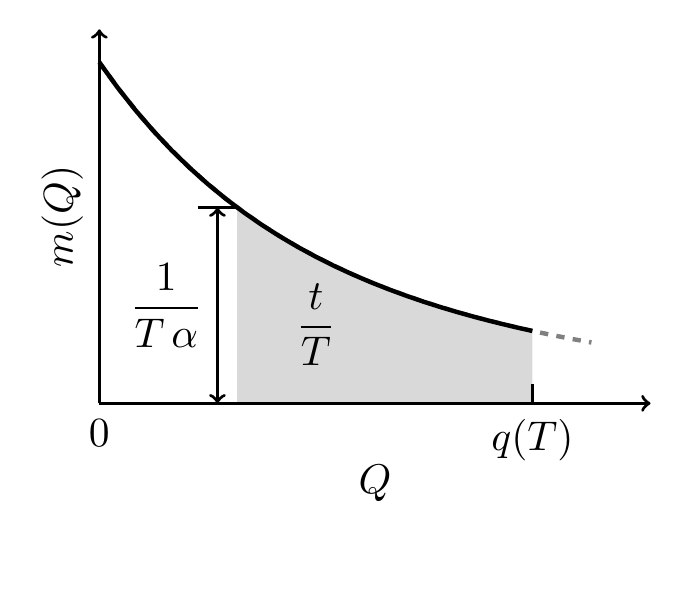
\begin{tikzpicture}[very thick, scale=2.5, every node/.style={scale=1.5}]
    % distribution
    \draw[domain=0:2.5, variable=\x, dashed, gray, ultra thick]
      plot({\x}, {sqrt(2*exp(-2*\x)+exp(-\x))});

    % shade
    \fill [gray!30!white, domain=0.7:2.2, variable=\x]
      (0.7, 0) --
      plot ({\x}, {sqrt(2*exp(-2*\x)+exp(-\x))})
      -- (2.2, 0) -- cycle;

    % thick curve
    \draw[domain=0:2.2, variable=\x, ultra thick]
      plot({\x}, {sqrt(2*exp(-2*\x)+exp(-\x))});

    % label for the shaded area
    \node[] at (1.1, 0.40) {$\dfrac{t}{T}$};

    \draw[<->] (0.6, 0)  --
               node[left, inner sep=1mm]
               {$\dfrac{1}{T \, \alpha}$}
               (0.6, 0.99488);
    % label for the ordinate
    %\node[fill=white] at (0.4, 0.7) {$\dfrac{1}{Ta}$};

    \draw[] (0.5, 0.99488) -- (0.7, 0.99488);
    \draw[->] (0, 0) -- node[below, inner sep=5mm] {$Q$} (2.8, 0);
    \draw[->] (0, 0) -- node[above, rotate=90] {$m(Q)$} (0, 1.9);

    % xtics
    \draw[] (0.0, 0.1) -- (0.0, 0.0) node[below] {$0$};
    \draw[] (2.2, 0.1) -- (2.2, 0.0) node[below] {$q(T)$};
  \end{tikzpicture}
  %\makebox[\linewidth][c]{
  %  \includegraphics[angle=0, width=0.9\linewidth]{fig/massq.pdf}
  %}
  \caption{
    \label{fig:massq}
    Geometric characterization of the optimal schedule,
    $\alpha(t)$,
    via the normalized mass distribution, $m(Q)$.
    %
    \note{
      The figure was produced by \texttt{tikz}.
      % Gnuplot version by doc/fig/massq.gp
    }%
  }
\end{center}
\end{figure}






\subsubsection{\label{sec:optinitalpha}
  Optimal initial updating magnitude
}


We now determine the optimal value of $q(T)$
that minimizes the total error defined in Eq. \eqref{eq:error_tot}.
%
We will consider simulations in which
the system is initially equilibrated at a
constant updating magnitude, $a_0$.
%
From Eqs. \eqref{eq:error_res}, \eqref{eq:xt2_eql1},
and \eqref{eq:error_asym2},
we find that
the optimal $q(T)$ satisfies
%
\begin{align}
  \frac{a_0}{2} \, M^2\bigl( q(T) \bigr)
  &+
  \sum_{k = 1}^{n-1}
  \lambda_k \, \epsilon_k \, e^{-2\lambda_k \, q(T)}
  \notag \\
  &= \frac{ M\bigl( q(T) \bigr) } { T } \int_0^{q(T)} M(Q') \, dQ'
  .
\label{eq:opt_qT}
\end{align}
%
%\begin{align}
%  m\bigl( q(T) \bigr)
%  +
%  \frac{2}{a_0 \, C \, M\bigl( q(T) \bigr)}
%  \sum_{k = 1}^{n-1}
%  \lambda_k \, \tilde u_k^2 \,
%  e^{-2 \, \lambda_k \, [a_0 \, T_0 + q(T)] }
%  \\=
%  \frac{1} { T \, (a_0 / 2) }
%  .
%\label{eq:opt_qT}
%\end{align}
%
\note{Let $q_T \equiv q(T)$,
$$
\begin{aligned}
  \frac{
    \partial \Err_R(T)
  }
  {
    \partial q_T
  }
  &=
  -a_0 \, M^2(q_T)
  -2
  \sum_{k=1}^{n-1} \lambda_k \,
  \tilde u_k^2 e^{-2 \, \lambda_k \, (a_0 \, T_0 + q_T)}
  ,
  \\
  \frac{
    \partial \Err_A(T)
  }
  {
    \partial q_T
  }
  &=
  \frac 2 T \,
  M(q_T) \,
  \int_0^{ q_T } M(Q) \, dQ
  =
  \frac{ 2 \, C } { T } \, M(q_T)
  .
\end{aligned}
$$
Then solve $\partial (\Err_R + \Err_A) / \partial Q_c = 0$.
}
%
We can rewrite the condition in terms of
the initial updating magnitude by Eq. \eqref{eq:mQ_invTa},
\begin{align}
  \alpha(0)
  =
  \frac{1}{T \, m\bigl( q(T) \bigr) }
  =
  \frac{ a_0 } { 2 }
  +
  \sum_{k = 1}^{n-1}
  \frac{
    \lambda_k \, \epsilon_k \, e^{-2\lambda_k \, q(T)}
  }{M^2\bigl( q(T) \bigr)}
  .
  \label{eq:opt_alpha0}
\end{align}
%
If the initial bias, $\epsilon_k$, is negligible, then
%
\begin{equation}
  \alpha( t = 0 )
  \approx
  \frac{ a_0 }
       { 2 }
  ,
\label{eq:half_alpha0}
\end{equation}
%
i.e. the optimal initial updating magnitude
is half of the equilibrium value.\footnote{This factor, $1/2$,
happens to coincide with the
recommended reduction factor of the updating magnitude
at stage transitions
in the original WL algorithm\cite{
wang2001, *wang2001pre}.
}


%For simulations with the same $a_0$,
%the shape of the mass distribution, $m(Q)$,
%also determines how much the optimal schedule
%would depend on the simulation length, $T$.
%%
%Since both $M(Q)$ and $m(Q)$ decrease monotonically with $Q$,
%Eq. \eqref{eq:opt_qT} shows that
%the optimal $q(T)$ increases with
%the simulation length, $T$,
%more so if $M(Q)$ has a long tail.
%%
%Thus, if $M(Q)$ decays slowly because of
%many near zero eigenvalues, $\lambda_k$'s,
%as in the metadynamics case,
%both the optimal schedule and
%normalized asymptotic error, $\Err_A(T) \cdot T$,
%would be sensitive to the simulation length, $T$.
%%
%In contrast, if all eigenvalues are $1.0$
%as in the single-bin or WL updating scheme discussed previously,
%the optimal schedule is
%given by the universal inverse-time formula,
%Eq. \eqref{eq:alpha_invt1},
%and the normalized asymptotic error
%is roughly a constant
%[cf. Eq. \eqref{eq:error_singlebin}].
%
%If $M(Q)$ decays rapidly,
%the distribution $m(Q)$ does not critically
%depend on the cutoff $q(T)$,
%once $q(T)$ is sufficiently large.
%%
%So the optimal schedules of these simulations
%approximately satisfy the scaling relations
%described in Sec. \ref{sec:mass_distr}.
%%
%If, however, $M(Q)$ has a long tail
%because of some near-zero $\lambda_k$'s,
%increasing the simulation length $T$
%generally alters the shape of the optimal schedule.




\subsubsection{\label{sec:band-matrix}
Homogeneous updating schemes}



Many commonly-used updating schemes,
such as the Gaussian updating scheme
used in metadynamics,
can be characterized by a rigid window
centered on the current bin.
%
For these translationally invariant or homogeneous
schemes, the eigenvalues can be readily found
from the window function ($\mu_0, \mu_1, \dots, \mu_b$)
as a cosine transform,
%
\begin{equation}
  \lambda_k
  =
  \mu_0
  +
  2 \,
  \sum_{ l = 1 }^b
  \mu_l
  \cos\left(
  \frac{ k \, l \, 2 \, \pi }
       {      g \, n        }
  \right)
  ,
  \label{eq:wband_eigenvalue}
\end{equation}
%
where $g = 1$ here for the periodic variable,
or $2$ for a non-periodic one
(cf. Appendix \ref{sec:more_wband}).



\subsubsection{\label{sec:procedure}
Procedure of computing the optimal schedule and error
}


Based on the above results,
we now give a procedure of computing
the optimal schedule and the error
for a given adaptive FDS simulation.
%
Basically, we need to extract
$\lambda_k$'s and $\Gamma_k$'s
from the given system and updating scheme (input),
and then apply them to Eq. \eqref{eq:q_opt}
for the schedule,
as shown in Fig. \ref{fig:vardep}.
%
%The dependence of variables are shown in Fig. \ref{fig:vardep}.
%
While the updating scheme alone
determines $\lambda_k$'s,
$\Gamma_k$'s depend also on the system
and the underlying sampling process.
%
We have

\begin{figure}[h]
\begin{singlespace}
  \fontsize{10pt}{\baselineskip}
  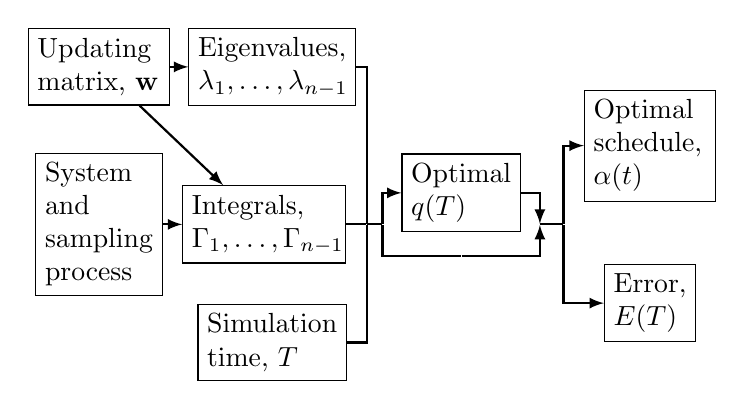
\begin{tikzpicture}
  \node[draw, text width={width("Updating ")}]
    (w) at (0, 3) {Updating \\matrix, $\mathbf w$};

  \node[draw, text width={width("sampling")}]
    (sys) at (0, 1) {System\\and\\sampling\\process};

  \node[draw, text width={width("Eigenvalues,")}]
    (lambda) at (2.2, 3) {Eigenvalues,\\$\lambda_1, \dots, \lambda_{n-1}$};

  \node[draw, text width={width("Integrals, iii")}]
    (gamma) at (2.1, 1) {Integrals, \\$\Gamma_1, \dots, \Gamma_{n-1}$};

  \node[draw, text width={width("Simulation")}]
    (T) at (2.2, -0.5) {Simulation\\time, $T$};

  \node[draw, text width={width("Optimal")}]
    (qT) at (4.6, 1.4) {Optimal\\ $q(T)$};

  \node[draw, text width={width("Schedule,")}]
    (alpha) at (7, 2) {Optimal schedule,\\ $\alpha(t)$};

    \node[draw, text width={width("Error,")}]
    (err) at (7, 0) {Error, $\Err(T)$};

  \node[inner sep=0, minimum size=0] (M1) at (3.4, 1) {};

  \node[inner sep=0, minimum size=0] (N1) at (5.9, 1) {};

  \node[inner sep=0, minimum size=0] (R1) at (3.6, 1) {};
  \node[inner sep=0, minimum size=0] (R2) at (4.6, 0.6) {};
  \node[inner sep=0, minimum size=0] (R3) at (5.6, 1) {};

  \draw[->, >=latex, thick]
    (w) edge (lambda)
    (w) edge (gamma)
    (sys) edge (gamma);

  \draw[->, >=latex, thick]
    (lambda) -| (M1)
    (gamma)  -- (M1)
    (T)      -| (M1)
    (M1)     -- (R1)
    (R1)     |- (qT);

  \draw[->, >=latex, thick]
    (qT)     -| (R3);

  \draw[->, >=latex, thick]
    (R3) -- (N1) |- (alpha);

  \draw[->, >=latex, thick]
    (N1) |- (err);

  \draw[->, >=latex, thick]
    %(M1) edge[bend left=70] (N1);
    (R1) |- (R2) -| (R3);
\end{tikzpicture}
\end{singlespace}
\caption{
  \label{fig:vardep}
  Dependence of variables in computing
  the optimal schedule and the error.
}
\end{figure}




\begin{enumerate}

\item
Compute the eigenvalues, $\lambda_k$'s
from the updating matrix, $\mathbf w$,
or from Eq. \eqref{eq:wband_eigenvalue}
for a homogeneous updating scheme.
%
Note that
the updating scheme should be stable
with no negative eigenvalue
(cf. the stabilization procedure in Appendix \ref{sec:stabilize_wband}).

\item \label{step:prerun}
Run a preliminary adaptive FDS simulation
%using the updating scheme
with constant updating magnitude, $a_0$.

\item \label{step:gamma}
Estimate $\Gamma_k$'s from Eq. \eqref{eq:varXt}
    (cf. Appendix \ref{sec:Gamma_measure})
    as well as the initial bias $\epsilon_k$.

\item \label{step:qT}
Compute the optimal value of $q(T)$ by solving Eq. \eqref{eq:opt_qT}.
%
We implemented a variant of the Newton-Raphson method\cite{press3rd}
(for $\ln q(T)$ to avoid negative values)
with the bisection method\cite{press3rd} as a fallback.
The initial value is set to $q(T) = \ln(1+T\,a_0/2)$.
%
%Since $m(Q)$ is a decreasing function of $Q$,
%we can start from an interval $[Q_L, Q_R]$
%that satisfies $m(Q_L) > 2/(T\,a_0) > m(Q_R)$
%(e.g. we can choose $Q_L = 0$,
%  and repeatedly double $Q_R$ until
%  the latter inequality is satisfied).
%%
%We can then iteratively refine the interval
%by substituting $Q_M = (Q_L + Q_R)/2$
%for either $Q_L$ and $Q_R$,
%depending on the sign of $m(Q_M) - 2/(T \, a_0)$,
%until the width of the interval is less than
%the desired precision,
%%
%and set $q(T)$ to $Q_M$.

\item \label{step:alpha}
Compute the optimal schedule by
  numerically integrating Eqs. \eqref{eq:q_opt} and \eqref{eq:mint}.
%
To handle Gaussian updating schemes more effectively,
  we have chosen the $\mathcal N+1$ grid points over $[0, q(T)]$ to be given by
  $q_{[i]} = \bigl(q(T) + 1\bigr) - \bigl(q(T)+1\bigr)^{1-i/\mathcal N}$,
  where $i = 0, \dots, \mathcal N$, and we chose $\mathcal N=20000$.
%
The curve $q(t)$ is then integrated
  using the trapezoidal rule\cite{press3rd},
  resulting in a list of values, $\bigl(q_{[i]}, t_{[i]} \bigr)$.
%
We then compute the updating magnitude by numerical differentiation:
  $\alpha_i = (1 - e^{-\lambda_1 \, \hat \alpha_i})/\lambda_1$
  and
  $\hat \alpha_i \equiv (q_{[i+1]} - q_{[i-1]}) / (t_{[i+1]} - t_{[i-1]})$,
  with
  $q_{[ -1]} \equiv 0$,
  $q_{[N+1]} \equiv q(T)$,
  $t_{[ -1]} \equiv 0$, and
  $t_{[N+1]} \equiv T$.
%
The resulting values of $(t_{[i]}, \alpha_{[i]})$
  can be linear interpolated
  to get the updating magnitude, $\alpha(t)$, at any simulation time, $t$.


\item
  Compute the total error $\Err(T)$ from
Eqs. \eqref{eq:error_tot},
  \eqref{eq:error_res},
  \eqref{eq:xt2_eql1},
  and
  \eqref{eq:error_asym2}.

\end{enumerate}

The above procedure is not always necessary.
%
As shown below, for a class of bandpass updating schemes,
  which resemble the Gaussian updating schemes,
  the asymptotically optimal schedule
  is simply given by the inverse-time schedule, Eq. \eqref{eq:alpha_invt1}.
%
For these updating schemes,
  the preliminary run with a constant updating magntiude
  can be replaced by the WL-style stagewise reduction
  until the updating magnitude falls under
  the value given the inverse-time prescription\cite{
    belardinelli2007, *belardinelli2007jcp, *belardinelli2008, *belardinelli2016}.



\subsection{\label{sec:cmpschemes}
Comparison of updating schemes}


Now that we can compute the optimal schedule
for a given updating scheme,
we will turn to the problem of finding
optimal updating schemes.


\subsubsection{\label{sec:optWL}
Asymptotic optimality of the single-bin scheme}



We will first show
that the single-bin scheme is asymptotically optimal.
%
Consider a class of $\mathbf w$ matrices
sharing the same set of eigenvectors,
hence the same $\Gamma_k$'s,
but with different positive eigenvalues,
$\lambda_k$'s.
%
Using the Cauchy-Schwarz inequality, we have,
for any set of nonnegative numbers, $c_k$'s\footnote{This
inequality follows from the nonnegativity of
the quadratic polynomial,
$$
\int_0^T
  dt \sum_{k = 1}^{n-1} \Gamma_k \,
    \left( {\dot y}_k \, \chi - c_k \right)^2
  \equiv
  A_2 \, \chi^2 + A_1 \, \chi + A_0
  ,
$$
which must carry a non-positive discriminant:
$A_1^2 - 4 \, A_0 \, A_2 \le 0$.},
%
%
\begin{align}
&
\left(
  \int_0^T dt
    \sum_{k = 1}^{n-1}
      \Gamma_k \, {\dot y}_k^2\bigl( q(t) \bigr)
\right)
%
\left(
  \int_0^T dt
    \sum_{k = 1}^{n-1}
      \Gamma_k \, c_k^2
\right)
%
\notag
\\
&
\qquad \qquad
\ge
\left(
  \int_0^T dt
    \sum_{k = 1}^{n-1}
      \Gamma_k \, c_k \, {\dot y}_k \, \bigl( q(t) \bigr)
\right)^2
\notag
\\
&
\qquad \qquad
=
\left(
  \sum_{k = 1}^{n-1} \Gamma_k \, c_k
    \left[
      1 - e^{ -\lambda_k \, q(T) }
    \right]
\right)^2.
\label{eq:CSineq}
\end{align}
%
Note that the last expression %of Eq. \eqref{eq:CSineq}
depends on the curve, $q(t)$ ($0 < t < T$),
only through the endpoint value, $q(T)$,
which is fixed in the variational process.
%
Thus, the inequality sets a lower bound
for the asymptotic error $\Err(T)$
given in Eq. \eqref{eq:error_asym}.
%
The equality is achieved
if $\dot y_k\left( q(t) \right) = c_k$
for all $k > 0$ at any $t$,
up to a multiplicative factor.
%
Solving these equations yields
%
\begin{equation}
  \alpha(t) = \frac{              1             }
                   { \lambda_k \, (t + t_{k0} ) },
\label{eq:alpha_invtk}
\end{equation}
with
\begin{equation}
  t_{k0} = \frac{             T            }
                { e^{ \lambda_k q(T) } - 1 }.
\label{eq:tk0}
\end{equation}
%
\note{Derivation.
  Integrating $\dot y_k = c_k$ yields
  \begin{equation}
    y_k(t) = c_k \left(t + t_{k0} \right).
  \tag{UK}
  \label{neq:ui_solution}
  \end{equation}
  Given that $y_k(T) = 1$ and $y_k(0) = e^{-\lambda_k \, q(T)}$,
  we have
  $$
  c_k = \frac{ 1 }{ T + t_{k0} },
  \quad
  \mathrm{and\;}
  \frac{ t_{k0} } { T + t_{k0} }
  =
  e^{ -\lambda_k \, q(T) }.
  $$
  Taking the logarithm of Eq. \eqref{neq:ui_solution} yields
  $$
  -\lambda_k \, q(T) + \lambda_k \, q(t)
  = \ln c_k + \ln \left( t + t_{k0} \right).
  $$
  Differentiating this with respect to $t$ yields
  Eq. \eqref{eq:alpha_invtk}.
}
%
Such a solution is possible only if
all nontrivial eigenvalues are equal,
%
%\begin{equation}
  $\lambda_1 = \dots = \lambda_{n-1}$.
%  \notag
%\end{equation}
%
Then, by Eq. \eqref{eq:tk0},
all $t_{k0}$'s also share the same value,
$t_0$,
such that
$y_k = (t + t_0) / (T + t_0)$,
and
$c_k = 1/(T + t_0)$
for $k > 0$.
%
The asymptotic error is then
%
\begin{align}
  \Err_A(T)
  =
  \frac{       T     }
       { (T + t_0)^2 }
  \sum_{ k = 1 }^{n-1}
    \Gamma_k
  .
\label{eq:error_asym_singlebin}
\end{align}
%
If we further assume $\lambda_1 = \cdots = \lambda_{n-1} = 1$,
%the optimal schedule given by
Eq. \eqref{eq:alpha_invtk}
recovers Eq. \eqref{eq:alpha_invt1}.
%

Since the first eigenmode represents
a uniform shift of the bias potential,
we can freely set $\lambda_0$ to be the same as $\lambda_1$
without changing the nature of the updating scheme.
%
Since an updating matrix
with identical eigenvalues
is a multiple of the identity matrix,
%
the corresponding updating scheme,
the single-bin scheme, is most efficient
in asymptotic convergence.
%if no eigenvalue $\lambda_k$ is zero.
%
%In Appendix \ref{sec:upperbound},
%we will show that the opposite limit of
%a set of well-separated eigenvalues
%will provide an upper bound for
%the asymptotic error, Eq. \eqref{eq:error_asym_ubound}.



\subsubsection{\label{sec:optscheme}
Bandpass updating schemes}


We can generalize
the single-bin scheme to a class of
perfect (brick-wall) \emph{bandpass} updating schemes
that ignore short-wavelength eigenmodes,
which are typically local noise.
%
Mathematically, these updating schemes
allow us to assign zero eigenvalues
to modes that are likely absent from the PMF.
%
For example,
%if we can assume
by assuming
that the PMF is sufficiently smooth
such that the eigenmodes can be limited to $k < K$,
%
we can construct an updating scheme with
$$
\lambda_0 = \cdots = \lambda_{K-1} = 1,
\mathrm{\; and \;}
\lambda_K = \cdots = \lambda_{n-1} = 0.
$$
%
Then, the updating matrix is given by
%
$$w_{ij} = n \sum_{k=0}^{K-1} \phi_{ki} \, \phi_{kj},$$
%
and Eq. \eqref{eq:error_asym_singlebin} is modified as
%
\begin{equation}
  \Err_A(T)
  =
  \frac {       T     }
        { (T + t_0)^2 }
  \sum_{ k = 1 }^{K-1}
    \Gamma_k.
%\notag
\label{eq:error_asym_sinc}
\end{equation}
%
The optimal schedule of these schemes
remains to be the inverse-time schedule
given by Eq. \eqref{eq:alpha_invt1},
%
with
%
\begin{equation}
  t_0
  =
  \frac{        1      }
       { \alpha(t = 0) }
  =
  \frac{  2  }
       { a_0 }
  ,
\label{eq:t0_sinc}
\end{equation}
%
where we have used Eq. \eqref{eq:half_alpha0}
in the second step.
%
\note{
For the single-bin updating scheme,
it recovers Eq. \eqref{eq:t0_singlebin}
under the assumption of Eq. \eqref{eq:xt2_eql}.
%
From Eq. \eqref{eq:xt2_eql}, we have
$$E(0) = \frac{1}{2} a_0 \sum_{k=1}^{n-1} \Gamma_k
= \frac{1}{2} \, a_0 \, \Gamma.$$
}
%
From Eqs. \eqref{eq:error_tot},
\eqref{eq:error_res},
\eqref{eq:tk0},
and
\eqref{eq:error_asym_sinc},
we get
%
\begin{equation}
  \Err(T)
  =
  \frac{   1     }
       { T + t_0 }
  \sum_{ k = 1 }^{ K - 1 }
    \Gamma_k
  .
\label{eq:error_sinc}
\end{equation}
%
This result recovers Eq. \eqref{eq:Emin_singlebin}
for the single-bin updating scheme:
if we set $K = n$, then\note{
  From Eq. \eqref{eq:eig_orthonormal_cols}, we have
  $\sum_{i=1}^n \rho_i \langle v_{*i}(t) \, v_{*i}(0) \rangle =\sum_{k=1}^{n-1} \langle {\tilde v}_k(t) \, {\tilde v}_k(0) \rangle.$
  Then sum over $t$ from $-\infty$ to $\infty$.
}
%
\begin{equation}
  \sum_{k=1}^{n-1} \Gamma_k
  = \sum_{i=1}^n \rho_i \, G_i = \Gamma
  ,
  \notag
  %\label{eq:Gamma_G_sum}
\end{equation}
%
This error is roughly proportional to the inverse simulation length,
as one would expect from an equilibrium FDS simulation.
%In Appendix \ref{sec:equilerr},
%we show that the above error tends
%to the error of the ideal equilibrium FDS simulation
%in the asymptotic limit.





%
%For example, consider a system that is initially
%prepared under a fixed $a_0$
%at the beginning of the schedule $\alpha(t)$.
%%
%Then for shorter times, $T \approx 0$,
%the error, dominated by the residual error
%given by Eq. \eqref{eq:error_res1},
%is clearly smaller if some eigenvalues
%are less than $1.0$ (the single-bin case).
%
%In practice, real simulations
%may have long achieved the desired precision
%before reaching the asymptotic regime,
%especially if the updating matrix
%has some $\lambda_k$'s close to $0$.




\section{\label{sec:results}
Numerical results}



\subsection{\label{sec:lj}Lennard-Jones}


Our test system is a Lennard-Jones (LJ) fluid of $N=100$ particles,
and we wish to compute the PMF along the distance of two special particles, $r$.
%
The two special particles are mutually non-interacting
but they interact normally with other particles,\footnote{they
have placed on an axis parallel to a side of the cubic box}
and the intrinsic distribution, $p^*$, is
the cavity distribution function, $y(r)$\cite{hansen}.
%
We will assume reduced units in this calculation.
%
The reference bias potential was pre-calculated from a long simulation.

We used the Metropolis algorithm for configuration sampling\cite{frenkel}.
%
Each step consists of
one MC trial for displacing one of the two special particles,
and another four trials for displacing the other particles.
%
In each trial, the displacement along each dimension is uniform,
with the size given by $0.1/\varrho^*$ to ensure the acceptance ratio is around 50\%,
where $\varrho^*$ is the reduced number density.


The PMF was calculated from $r = 0$ to half of the box dimension
on a grid of size $\Delta r = 0.01$ in reduced units.
%
Two densities were tried, $\varrho^* = 0.1$ and $0.8$,
and the numbers of bins were $500$ and $250$, respectively.
%
We tested the single-bin, Gaussian, and bandpass updating schemes.
%
Each simulation started with an ``equilibration'' phase
of $10^7$ steps with a fixed updating magnitude, $a_0 = 10^{-4}$,
followed by a production phase
with updating magnitude given by
either the inverse-time or optimal schedule.
%
We repeated each simulation multiple times
and report the average.
%
To make sure the same schedule for multiple runs under the same condition,
the optimal schedule was pre-computed from a set of fixed values of
$\Gamma_k$ and $\epsilon_k$,
although they can also be fairly accurately estimated from the data
collected from the equilibration phase of each individual run.



As shown in Table 1,
both the inverse-time and optimal schedule reduced
the error significantly,
and the errors roughly matched the predicted values
calculated from the precomputed $\Gamma_k$'s and $\epsilon_k$'s.
%
The Gaussian scheme appeared to be superior
to the single-bin scheme in the $\varrho^* = 0.1$ case,
but not in the $\varrho^* = 0.8$ case.
%
In either case, there was an optimal width of Gaussian
(which was $\sigma = 0.37$ for $\varrho^* = 0.1$
or $0.07$ for $\varrho^* = 0.8$ in this case),
an overly large width could be counterproductive.

In Fig. \ref{fig:lj_xerr},
we show the error components against the eigenmode index
for the Gaussian updating scheme of width $\sigma = 0.2$.
%
While the Gaussian updating scheme effectively suppressed
the initial errors for short-range (large $k$) modes,
it also slowed down the reduction of errors of these modes.
%
As a result, the final errors of the long-range (small $k$) modes
were larger than those from the single-bin scheme.
%
For the Gaussian updating scheme
the inverse-time schedule tended to reduce the updating magnitude too rapid
leaving a hump on the error profile for the middle-range modes.
%
The optimal schedule improved over the inverse-time schedule
and produced a flatter profile for the final error.
%
It is also possible to roughly
recover the single-bin result by using the correction formula
based on the histogram, Eq. \eqref{eq:UHcorr}.
%
This correction usually improves the accuracy of the small $k$ modes
but not necessarily for the large $k$ modes.


In Fig. \ref{fig:lj_alpha}. 
we show the optimal schedules in a few cases.
%
Generally, the optimal schedule
for the $\varrho^* = 0.8$ case
was closer to the inverse-time schedule
than that for the $\varrho^* = 0.1$ case.
%
This was probably because in the former case
the first mode dominates the total error,
$\Gamma_1 \approx \Gamma$,
and the schedule was roughly optimized for this mode,
resulting in
$\alpha(t) \approx 1/[\lambda_1 (t + t_0)] \approx 1/(t+t_0)$
as $\lambda_1 \approx 1$
[especially when width of the Gaussian is small,
cf. Eq. \eqref{eq:lambda_Gaussian}].
%
Since we have chosen a long equilibration period
for preliminary run with a constant updating magnitude,
the starting magnitude was usually around $a_0/2 = 5\times10^{-5}$
[cf. Eq. \eqref{eq:half_alpha0}].
%
But if the Gaussian is too wide,
such as the $\sigma = 0.6$ case,
the eigenvalues $\lambda_k$ of some modes
became too small to damp out the initial bias,
resulting in nonnegligible $\epsilon_k$,
and much larger initial updating magnitude, $\alpha(0)$
[cf. Eq. \eqref{eq:opt_alpha0}].
%
In this case, our method would fail
because the resulting bias potential would no longer be small.


\begin{table}[h]\footnotesize
  \caption{\label{tab:error_LJ}
    Error of the LJ system.
    The numbers have been averaged over multiple runs,
    and the numbers in parentheses are predicted values;
    $\Err_\mathrm{init.}$
    denotes the error
    at the end of the equilibration phase with a constant magnitude;
    $\Err_\mathrm{final}$
    denotes the error at the end of the production phase under
    either the inverse-time ($1/t$) or optimal schedule (opt.).
    \note{The reference values can be found on the second line of \texttt{verr.log}.}
  }
  \setlength{\tabcolsep}{2pt}
  \renewcommand\arraystretch{1.4}
  \begin{tabular} { l c c c c }
    \hline
    Scheme & Sched. &
    $\Err_\mathrm{init.}$ &
    $\Err_\mathrm{final}$
    \\
    \hline
    \multicolumn{4}{c}{
      $\varrho^* = 0.1$,
      $500$ bins,
      $\Gamma_1 \approx 111$,
      $\Gamma \approx 1.1\times10^3$.
    } \\
    \hline
    single-bin & $1/t$
    & $5.7(5.7)\times10^{-2}$
    & $9.1(11.4)\times10^{-5}$
    \\
    %\hline
    $\sigma=0.1$ & $1/t$
    & $7.7(8.9)\times10^{-3}$
    & $6.8(8.2)\times10^{-5}$
    \\
    %\hline
    $\sigma=0.1$ & opt.
    & $7.6(8.9)\times10^{-3}$
    & $3.2(3.9)\times10^{-5}$
    \\
    %\hline
    $\sigma=0.2$ & $1/t$
    & $6.5(7.8)\times10^{-3}$
    & $4.0(4.8)\times10^{-5}$
    \\
    %\hline
    $\sigma=0.2$ & opt.
    & $7.0(7.8)\times10^{-3}$
    & $2.5(2.8)\times10^{-5}$
    \\
    %\hline
    $\sigma=0.5$ & $1/t$
    & $5.5(6.6)\times10^{-3}$
    & $3.2(3.8)\times10^{-5}$
    \\
    %\hline
    $\sigma=0.5$ & opt.
    & $5.8(6.6)\times10^{-3}$
    & $2.6(3.0)\times10^{-5}$
    \\
    %\hline
    $K=20$ & $1/t$
    & $8.1(8.9)\times10^{-3}$
    & $1.6(1.8)\times10^{-5}$
    \\
    \hline
    \multicolumn{4}{c}{
      $\varrho^* = 0.8$,
      $250$ bins,
      $\Gamma_1 \approx 2.0\times10^4$,
      $\Gamma \approx 2.7\times10^4$
    } \\
    \hline
    single-bin & $1/t$
    & $1.3(1.4)$
    & $2.7(2.7)\times10^{-3}$
    \\
    %\hline
    $\sigma=0.1$ & $1/t$
    & $1.3(1.3)$
    & $2.9(2.8)\times10^{-3}$
    \\
    %\hline
    $\sigma=0.1$ & opt.
    & $1.2(1.3)$
    & $2.8(2.8)\times10^{-3}$
    \\
    %\hline
    $\sigma=0.2$ & $1/t$
    & $1.3(1.2)$
    & $3.4(3.2)\times10^{-3}$
    \\
    %\hline
    $\sigma=0.2$ & opt.
    & $1.2(1.2)$
    & $3.1(2.9)\times10^{-3}$
    \\
    %\hline
    $\sigma=0.5$ & $1/t$
    & $0.9(0.9)$
    & $9.8(8.0)\times10^{-3}$
    \\
    %\hline
    $\sigma=0.5$ & opt.
    & $1.0(0.9)$
    & $5.8(5.4)\times10^{-3}$
    \\
    %\hline
    $K=20$ & $1/t$
    & $1.3(1.3)$
    & $3.0(2.7)\times10^{-3}$
    \\
    \hline
  \end{tabular}
\end{table}



\begin{figure}[h]
\begin{center}
  \makebox[\linewidth][c]{
    \includegraphics[angle=0, width=1.0\linewidth]{fig/lj_xerr.pdf}
  }
  \caption{
    \label{fig:lj_xerr}
    Error components for the FDS simulation on the LJ system
    using the Gaussian updating scheme with width $\sigma = 0.2$.
    %
    The optimal schedule (opt.) is more effective
    in reducing the errors of middle-range modes
    than the inverse-time ($1/t$) schedule.
    The lines are a guide to the eyes.
  }
\end{center}
\end{figure}



\begin{figure}[h]
\begin{center}
  \makebox[\linewidth][c]{
    \includegraphics[angle=0, width=1.0\linewidth]{fig/lj_alpha.pdf}
  }
  \caption{
    \label{fig:lj_alpha}
    Optimal schedule of the Gaussian updating scheme
    for the LJ system.
    %
    The starting updating magnitude was usually
    around $a_0/2 = 5\times10^{-5}$
    as given by Eq. \eqref{eq:half_alpha0}.
    But an overly wide Gaussian window ($\sigma = 0.6$)
    resulted in a much larger updating magnitude.
  }
\end{center}
\end{figure}











\section{\label{sec:conclusion}
Conclusions and Discussions}



In conclusion,
we have proposed a method of computing
the optimal schedule of the updating magnitude
for a general class of free energy calculation methods,
which we refer to as adaptive flat-distribution-sampling (FDS) methods
that include the Wang-Landau (WL) algorithm and metadynamics.
%
Adaptive FDS methods
incrementally update a bias potential
along a collective variable
to offset the potential of mean force (PMF)
and thereby sample a flat distribution.
%
The optimal schedule delivers the fastest convergence
of the bias potential,
and thus helps minimize the effort
of computing the PMF.
%They differ by the updating schemes,
%which specify how the bias potential is modified
%in each updating step.
%%
%In the single-bin or WL case,
%the update is limited to the current bin;
%while metadynamics,
%the bias potential of a neighborhood of the current one
%is updated with relative weight specified by a Gaussian window.


The optimal schedule depends on the updating window function,
which can be limited to a single-bin (as often in the WL case),
or extended to several neighboring bins
taking a Gaussian shape (as often in the metadynamics case).
%
More generally,
each adaptive FDS method is associated with
an updating scheme
that can be mathematically characterized
by an updating matrix.
%
Each column of the matrix gives the normalized
window function for the bin corresponding to the column.
%
Our method computes the optimal schedule from
the eigenvalues of the updating matrix,
and the integrals of the autocorrelation functions
of the eigenmodes.
%
For the single-bin scheme,
we confirmed that the optimal schedule
is given by the inverse-time formula,
Eq. \eqref{eq:alpha_invt1}.
%
For a general multiple-bin scheme,
including the Gaussian one,
the optimal schedule is not given by a simple closed form,
but is implicitly given by an equation of motion
of a free particle with a position-dependent mass, Eq. \eqref{eq:q_opt}.
%
In this case,
the optimal schedule and error
can be sensitive to the simulation length.
%
%The initial updating magnitude is always
%half of the previous equilibrium value.
% the value used during equilibration.

We have also shown that
the single-bin scheme is optimal
in the long time limit
without a priori assumptions
about the smoothness of the PMF.
%
However, if some eigenmodes
correspond to local noise
that is expected to be absent from the PMF,
we can construct a
class of bandpass updating schemes
that are also optimal for asymptotic convergence.
%
The optimal schedule of these bandpass schemes
is always given by an inverse-time formula.

We believe that one of the main appeals
of the Gaussian updating scheme
is its ability to maintain a smooth bias potential,
which is useful for MD applications.
%
However, it requires a careful choice of the width and
a sufficiently long equilibration phase under constant updating magnitude.
%
For reasonable parameters,
one may use the histogram correction, Eq. \eqref{eq:UHcorr},
in a post-simulation analysis
to recover the possible accuracy loss
and obtain a bias potential similar to
that from the optimized single-bin scheme.
%%
%However, the performance gain
%is relatively small for short simulations
%with a local sampling process such as MD.



The analysis in this study has two limitations.
%
First, we have ignored the \emph{systematic}
error\cite{zhou2005, morozov2007, zhou2008}
caused by the updates in adaptive FDS methods.
%
This is valid in the asymptotic regime:
when the updating magnitude is small
and the sampling is a quasi-equilibrium one\cite{
  zhou2005, morozov2007, zhou2008, barducci2008, dama2014},
the random error,
which is roughly proportional to
the square root of the updating magnitude\cite{
  zhou2005, morozov2007, zhou2008, bussi2006},
can easily outweigh
the systematic error,
which is roughly proportional to
the magnitude itself\cite{morozov2007}.
%
%Our method of analysis is most useful for long simulations
%to achieve relatively precise results.
%
Second, by using the white noise approximation,
we have represented the autocorrelation function
of each eigenmode by a single number, $\Gamma_k$.
%
Although this assumption appeared to work well
on our test system for modeling long simulations,
they may break down for relatively short simulations
of glassy systems.
%Our immediate interest is to apply these relations to
%problems containing aqueous mixtures of proteins and nucleic acids.


\section{Acknowledgments}

We thank Dr. Y. Mei, J. Wang,
O. Nassar, Dr. C. Lai, Dr. S. Ou, D. Stuhlsatz,
Dr. C. Myers, and Dr. O. Samoylova
for helpful discussions.
%
We gratefully acknowledge the Robert A. Welch Foundation (H-0037),
the National Science Foundation (CHE-1152876)
and the National Institutes of Health (GM-037657)
for partial support of this work.
%
JM thanks support from the National Institutes of Health (R01-GM067801, R01-GM116280),
the Welch Foundation (Q-1512),
and National Science Foundation (Grant PHY-1427654).
%
This research used computing resources of the National Science Foundation XSEDE grid.
%
%


\appendix




\section{\label{sec:equilerr}
Runtime average interpretation
of the inverse-time schedule
}


The optimality of the inverse-time schedule can be considered
as a natural consequence of the stabilization of a runtime average
as the sample size increases\cite{
  marsili2006, barducci2008}.
%
%We first note that a runtime average
%\begin{equation}
%  X(t) = \frac{x(1) + \cdots + x(t)}{t}
%  .
%  \label{eq:avx}
%\end{equation}
%can be written as a recurrence relation
%\begin{equation}
%  X(t) = X(t - 1) + \frac{x(t) - X(t-1)}{t}
%  .
%  \label{eq:avx_recur}
%\end{equation}
%%
%Here $x(t) - X(t-1)$ serves as an independent correction
%from data point at time $t$ to the previous average value,
%and this correction is absorbed into the average
%with a weight of $1/t$,
%which is the inverse sample size.

%We can use Eq. \eqref{eq:avx_recur} to incrementally
%improve the estimated
%bias potential given by Eq. \eqref{eq:vcorr_equil}.
%
Assuming that we can linearize the histogram correction
in Eq. \eqref{eq:vcorr_equil} as
$\ln x \approx x - 1$ % (for $x \approx 1$),
and apply it to the instantaneous histogram, $h_i(t)$,
then the independent estimate of bias potential in each step
is given by
%
\begin{equation*}
  \hat u_i(t) \approx u_i(t) + \frac{ h_i(t) } { p_i } - 1
  .
  \label{eq:uhatt}
\end{equation*}
%
The time average
$\hat U_i(t) \equiv (1/t) \sum_{\tau=1}^t \hat u_i(\tau)$
is
\begin{align}
  \hat U_i(t)
  &\approx
  \frac{1}{t} \sum_{\tau=1}^t
  \left[
    u_i(\tau) + \frac{ h_i(\tau) } { p_i } - 1
  \right]
  .
  \label{eq:Uhatt}
\end{align}
%
For a fixed bias potential, the above formula
recovers the linearize Eq. \eqref{eq:vcorr_equil}.
%
But with the single-bin updating scheme,
Eq. \eqref{eq:wl_update}
we have, up to a constant shift,
%
\begin{align}
  \hat U_i(t)
  &\approx
  \frac{1}{t} \sum_{\tau=1}^t
  \left[
    u_i(\tau) +
    \frac{ u_i(\tau + 1) - u_i(\tau) } { \alpha(t) }
  \right]
  ,
  \notag
  \\
  &\approx
  \Delta u_i
  +
  \sum_{\tau=1}^t
  \left[
    1 + \frac{1}{\alpha(\tau - 1)} - \frac{1}{\alpha(\tau)}
  \right]
  \frac{ u_i(\tau) } {t}
  ,
  \label{eq:Uhat_sum}
\end{align}
where
$$
\Delta u_i \equiv \frac{u_i(t+1)}{t \, \alpha(t)}
- \frac{u_i(1)}{t \, \alpha(0)}.
$$
%
With the inverse-time schedule, Eq. \eqref{eq:alpha_invt},
each term in the square brackets vanishes,
and if we further define $\alpha(0) \to \infty$
$$
u_i(t+1) = \hat U_i(t),
$$
the bias potential represents
the runtime average of the correction, $\hat u_i(t)$.
%
Another special case is $\alpha(\tau) = 0$ for $\tau = 0, 1, \dots$,
then Eq. \eqref{eq:Uhat_sum} is reduced to a plain average
$$
\hat U_i(t) \approx \frac 1 t \sum_{\tau=1}^t u_i(\tau).
$$
where we have assumed an equilibrium condition
such that $u_i(t+1) \approx u_i(1)$.

For other updating schemes and schedules, we may still use
Eq. \eqref{eq:Uhatt} to construct a correction:
%
\begin{align}
  \hat U_i(t)
  &\approx
  U_i(t)
  +
  \frac{ H_i(t) } { p_i } - 1
  \approx
  U_i(t)
  +
  \ln \frac{ H_i(t) } { p_i }
  ,
  \label{eq:UHcorr}
\end{align}
%
where
\begin{align}
  U_i(t)
  &= \frac 1 t \sum_{\tau = 1}^t u_i(\tau)
  ,
  \notag
  %\label{eq:uav_def}
  \\
  H_i(t)
  &= \frac 1 t \sum_{\tau = 1}^t h_i(\tau)
  .
  \label{eq:hav_def}
\end{align}
%
%Thus, the bias potential from a WL simulation
%(which typically uses the single-bin updating scheme)
%under the inverse-time schedule
%would reach a similar precision
%as an ideal multicanonical simulation
%with fixed and nearly perfect bias potential.
%the precision at long times.
%%
%Thus, it is unnecessary to fix the bias potential
%after an adaptive FDS simulation has reached
%sufficiently convergent just for better precision
%of the final PMF.



%Second,
%it shows close connection between
%the WL algorithm under the inverse-time schedule
%and self-healing umbrella sampling.
%In the latter,
%the bias potential is computed from
%a weighted runtime average of the histogram\cite{
%  marsili2006, barducci2008},
%which is analogous to the adaptive bias force method\cite{
%  darve2001, *darve2008}.
%
%Third,
%it also relates a WL simulation under the inverse-time schedule
%to a time-averaged variant of the regular WL simulation.
%%
%In the variant, the updating magnitude is fixed,
%but the bias potential over the simulation course is averaged
%as the final result\cite{zhou2005}.
%%
%The above demonstration shows that the inverse-time schedule
%has already effectively implemented an implicit average
%so that no explicit averaging is needed in the former approach.
%%
%The inverse-time schedule approach is preferred, however,
%because with a decreasing updating magnitude,
%it minimizes the systematic error caused by
%the on-the-fly updating scheme\cite{
%  zhou2005, zhou2008},
%which is ignored in this analysis.




\section{\label{sec:wltoinvt}
Inverse-time schedule as the optimal limit of the WL algorithm}


We may understand the inverse-time schedule %, Eq. \eqref{eq:},
as an optimal limit of the stage-wise WL updating scheme.
%
%Our calculation below will focus on the one-variable problem,
%as in Sec. \ref{sec:onevar}.

To begin, we split the entire simulation into $S$ stages,
each with a fixed magnitude, $\alpha_s$ ($1 \le s \le S$).
%
We denote the number of steps in stage $s$ as $T_s$, and
$\sum_{s=1}^S T_s = T$.
%
%\begin{equation}
%  \sum_{s = 1}^S T_s = T
%  ,
%  \label{eq:sumT}
%\end{equation}
%
We assume that
the magnitude follows geometrically,
%
\begin{equation}
  \alpha_s = \alpha_0 \, r^s
  ,
  \label{eq:alphas}
\end{equation}
%
with $0 < r < 1$.
%
%and that the system is properly equilibrated
%under a constant magnitude initially.
%
We wish to find the best distribution of the simulation time
into the $S$ stages
as well as
the optimal number of stages and $r$.


If we denote the error at the end of stage $s$ as $E_s$,
then $q\left( \tau^{(s)} \right) = \alpha_s \, \tau^{(s)}$,
where $\tau^{(s)}$ denotes the number of steps in stage $s$,
and from Eq. \eqref{eq:ET_average}, we have
%
\begin{align}
  E_s
  &=
  E_{s - 1} \, e^{-2 \, \alpha_s \, T_s }
  +
  \Gamma \, \int_0^{T_s}
  \alpha_s^2 \,
  e^{ -2 \, \alpha_s \, \left(T_s - \tau^{(s)}\right) }
  \, d \tau^{(s)}
  \notag
  \\
  &=
  \left(
    E_{s - 1} - \frac{ \Gamma \, \alpha_s } { 2 }
  \right)
  e^{ - 2 \, \alpha_s \, T_s }
  +
  \frac{ \Gamma \, \alpha_s } { 2 }
  .
  \label{eq:errorstage}
\end{align}
%
Our aim is to minimize the error
of the final stage, $E_S$.
%
To do so, let us consider shifting simulation time
by $\delta T$ from
stage $s+1$ to stage $s$,
then $E_{s+1}$ is affected as
%
\begin{align*}
  \delta E_{s+1}
  =
\left[
  2 \, \alpha_{s+1}
  \left(
    E_s - \tfrac{ \Gamma \, \alpha_{s+1} } { 2 }
  \right)
  +
  \frac{ \partial E_s } { \partial T_s }
\right]
e^{-2 \, \alpha_{s+1} \, T_{s+1} }
\,
\delta T
.
\end{align*}
%
Since this variation does not directly affect the error of later stages,
the above expression must be zero to minimize the final error, i.e,
%
\begin{align*}
  2 \, \alpha_{s+1}
  \left(
    E_s - \frac{ \Gamma \, \alpha_{s+1} } { 2 }
  \right)
  &=
  -\frac{ \partial E_s } { \partial T_s }
  %\\
  %&=
  %2 \, \alpha_s \, e^{-2 \, \alpha_s \, T_s}
  %\left(
  %  E_{s-1} - \frac{ \Gamma \, \alpha_s } { 2 }
  %\right)
  %\\
  =
  2 \, \alpha_s \, \left(E_s - \frac{ \Gamma \, \alpha_s } { 2 }  \right)
  ,
\end{align*}
%
where we have used Eq. \eqref{eq:errorstage}
in the second step.
%
Thus,
\begin{equation}
  E_s
  =
  \frac{ \Gamma } { 2 } \, ( \alpha_s + \alpha_{s+1} )
  =
  \frac{ \Gamma } { 2 } \, \alpha_s ( 1 + r )
  .
  \label{eq:Es}
\end{equation}
%
Using Eqs. \eqref{eq:Es} and \eqref{eq:alphas}
in Eq. \eqref{eq:errorstage}, we get
%
\begin{equation}
  e^{-\alpha_s \, T_s } = r
  .
  \label{eq:exp_r}
\end{equation}
%

To compute the optimal schedule,
we map the overall simulation time, $t$,
to the stage number, $s$, as
%
\begin{align*}
  t
  = \sum_{s' = 1}^s T_{s'}
  = \frac{ 1 - r^s } { 1 - r } \, T_s
  = \frac{ 1 } { \gamma } \,
  \left(
    \frac{1}{\alpha_s}
    -
    \frac{1}{\alpha_0}
  \right)
  ,
\end{align*}
where
$\gamma = ( 1 - r ) / \ln(1/r)$,
and we have used Eq. \eqref{eq:exp_r} in the last step.
%
Thus,
%
\begin{equation}
  \alpha_s =
  \frac{ 1 }
  { \gamma \, t + \alpha_0^{-1} }
  ,
  \label{eq:alphas_t}
\end{equation}
%
and the final error is given by
%
\begin{align}
  E_S
  =
  \frac{\Gamma}{2}
  \frac{ 1 + r }
  { \gamma \, T + \alpha_0^{-1} }
  ,
  \notag
\end{align}
%
which is minimized as $r \to 1$
for a large $T$
(at this point, $\gamma \to 1$).
%
\note{
  For a large $T$, $E_S \approx \frac{\Gamma}{2T} \frac{1+r}{\gamma}$.
  Define $\delta = 1 - r$,
  we have $1/\gamma = 1+ \delta/2 + \delta^2/3 + \cdots$,
  and
  $$
  \frac{1+r}{\gamma}
  =
  (2 - \delta)
  \left(
  1 + \frac{\delta}{2} + \frac{\delta^2}{3} + \cdots
  \right)
  =
  2 + \sum_{n=1}^\infty \frac{n-1}{n(n+1)}\delta^n \ge 2
  .
  $$
}
%
If we identify the parameter, $\alpha_0$,
as the initial updating magnitude, $\alpha(t = 0)$,
then this result agrees with Eq. \eqref{eq:t0_sinc},
with $t_0 = \alpha_0^{-1}$,
and the schedule given by Eq. \eqref{eq:alphas_t}
is identical to that from Eq. \eqref{eq:alpha_invt1}.




\section{\label{sec:hfluc}
Histogram fluctuation}


Here we wish to show that for an FDS simulation
with a nearly-perfect bias potential
(e.g. a long WL simulation under the single-bin updating scheme
with the inverse-time schedule),
the histogram fluctuation
is roughly equal to the final error.
%
First, in the long time limit, the fluctuation of
the instantaneous histogram is dominated by the random part,
%
\begin{equation}
  \xi_i(t) \approx \zeta_i(t)
  ,
  \label{eq:xi_zeta}
\end{equation}
and we would have for the Fourier transform,
$\tilde \xi_k(t) \approx \tilde \zeta_k(t).$
%
If we define the time average,
$$
\tilde \Xi_k(T) \equiv \frac 1 T \sum_{t = 1}^T \tilde \xi_k(t)
=\mathcal F\left[ \frac{ H_i } { p_i } \right]_k
,
$$
then the histogram fluctuation of mode $k$ is given by
$\left\langle \tilde \Xi_k^2(T) \right\rangle$,
and from Eq. \eqref{eq:xi_zeta}, we have
\begin{align*}
\left\langle \tilde \Xi_k^2(T) \right\rangle
&=
\frac{1}{T}
\sum_{t=-\infty}^\infty
\left\langle
  \tilde \xi_k(t) \, \tilde \xi_k(0)
\right\rangle
\\
&\approx
\frac{1}{T}
\sum_{t=-\infty}^\infty
\left\langle
  \tilde \zeta_k(t) \, \tilde \zeta_k(0)
\right\rangle
=
\frac{ \Gamma_k } { T }
.
\end{align*}
%
The total histogram fluctuation is
$$
F(T)
=
\sum_{k=1}^{n-1} \left\langle \tilde \Xi_k^2(T) \right\rangle
=
\frac{ \Gamma } { T }.
$$
%
Comparing this to Eq. \eqref{eq:Emin_singlebin},
we conclude
\begin{equation}
  F(T+t_0) \approx E(T)
  .
  \notag
  %\label{eq:fluc}
\end{equation}
%and the histogram fluc
%serves as a good estimate of the final error.
%
\note{
Note that the expected histogram flatness
was previously used to define the error\cite{zhou2005, zhou2008},
and the above demonstration shows the definition
is compatible with ours, Eq. \eqref{eq:error_def}, in the long-time limit.
An interesting application\cite{zhou2008},
of the above result is
to set the updating magnitude by $F/\Gamma$
for some empirical value [$\Gamma \approx 10$ there, see Eq. (8)]
as a substitute of the inverse-time schedule.
}




\section{\label{sec:Gamma_measure}
Measurement of the integrals of the autocorrelation functions of the eigenmodes
}



Here we give a method of measuring
the integrals of the autocorrelation functions, $\Gamma_k$'s,
in an adaptive FDS simulation
with a constant updating magnitude.
%
This method has the advantage of not requiring
explicit computation of 
the autocorrelation functions of the eigenmodes.
%
The basic idea is to use Eq. \eqref{eq:xt2_eql}.
%
However,
without knowing the intrinsic distribution, $p^*_i$,
we cannot compute the shifted bias potential, $v_i$.
%
The problem can be avoided by replacing the shift
by the time average of the bias potential.

We first note that the difference, 
$u_i(t) - v_i(t) = \ln(p^*_i/p_i)$, is a constant of time,
so is its Fourier transform,
$\tilde u_k(t) - \tilde v_k(t)$.
%
It follows that
${\tilde u}_{k}$ and ${\tilde v}_{k}$ would also share the same variance.
%
But since the ensemble average of ${\tilde v}_{k}$
is zero, we have
\begin{equation*}
  \operatorname{var} {\tilde u}_{k}
  =
  \operatorname{var} {\tilde v}_{k}
  =
  \left\langle {\tilde v}_{k}^2 \right\rangle
  .
\end{equation*}
%
Finally, by using Eq. \eqref{eq:xt2_eql},
we get
%
\begin{equation}
  \operatorname{var} {\tilde u}_k
  =
  \frac{1}{2} \,
  a_0 \, \Gamma_k \, \lambda_k,
\label{eq:varXt}
\end{equation}
%
where the variance can be computed from trajectory averages.
%
A practical limitation is that Eq. \eqref{eq:varXt}
would fail if some eigenvalue, $\lambda_k$, is close to zero.
So it is best used for the single-bin updating scheme.




\section{\label{sec:more_wband}
Homogeneous updating schemes
}


Here, we give some details
on the homogeneous updating schemes.
%
By the translational invariance,
these schemes
satisfy detailed balance,
Eq. \eqref{eq:w_detailedbalance},
for the flat distribution, $\rho_i = 1/n$,
i.e. the updating matrix, $\mathbf w$,
is symmetric.
%
The updating matrices
share the same set of eigenvectors
(which here are sines and cosines of different frequencies),
and thus are completely determined
by the eigenvalues.
%
Further, the multiplication of $\mathbf w$
can be reduced to a convolution with the window function,
or the updating kernel.
%
Thus,
there is a one-to-one correspondence between
the eigenvalues of $\mathbf w$
and the updating kernel.



\subsection{\label{sec:wband_eig}
Eigenvalues and eigenvectors}

%\subsubsection{\label{sec:bandkernel}
%Updating kernel and eigenvalues}



%While translationally-invariant
%updating schemes
%naturally suit periodic variables\cite{
%dama2014},
%they can also be extended to non-periodic variables
%by imposing the reflective boundary condition\cite{
%bussi2006}.
%%
%For simplicity, we will assume that the target
%distribution is flat, or $p_i = 1/n$, below.



For a periodic variable\cite{dama2014},
the updating matrix, $\mathbf w$,
assumes the following form
%
\begin{equation}
  w_{ij}
  =
  \mu_{i-j}
  +
  \mu_{i-j+n}
  +
  \mu_{i-j-n}
  ,
\notag
%\label{eq:w_band_pbc}
\end{equation}
%
where the numbers,
$\mu_{-b}, \dots, \mu_b$, ($b \le n/2$)
characterizing the rigid window
will be referred to as an \emph{updating kernel}\cite{bussi2006}.
%
To satisfy Eq. \eqref{eq:w_sumj},
we impose the normalization
%
\begin{equation}
  \mu_{-b} + \cdots + \mu_b = 1
  ,
\label{eq:mu_normalization}
\end{equation}
%
with $\mu_l = 0$ for $|l| > b$.
%
If $b = n/2$, $\mu_{-b}$ is removed
from the sum in Eq. \eqref{eq:mu_normalization}
to avoid double counting.
%
For simplicity, we also impose the symmetry
%
\begin{equation}
  \mu_i = \mu_{-i}
  .
\label{eq:mu_symm}
\end{equation}


To find the eigenvectors,
we define for a periodic variable, $\phi_i$,
the out-of-boundary values by
%
\begin{equation}
  \phi_j = \phi_{j \pm n},
\label{eq:phi_pbc}
\end{equation}
%
such that $j \pm n$ lies in between $1$ and $n$.
%
Then, the multiplication of the matrix, $\mathbf w$,
is equivalent to a convolution with the kernel:
%
\begin{equation}
  \sum_{ j = 1 }^n
    w_{ij} \, \phi_j
  =
  \sum_{ j = 1 - n }^{ 2 \, n }
    \mu_{i - j} \, \phi_j
  =
  \sum_{ l = -b }^{ b }
    \mu_l \, \phi_{ i - l}
  .
\label{eq:wmul_to_convol}
\end{equation}
%
\note{The derivation of the first step of
  Eq. \eqref{eq:wmul_to_convol}:
$$
\begin{aligned}
  \sum_{j = 1}^n
    w_{ij} \, \phi_j
  &=
  \sum_{j = 1}^n
    \mu_{i - j} \, \phi_j
  +
  \sum_{j = 1}^n
    \mu_{i - j - n} \, \phi_j
  +
  \sum_{j = 1}^n
    \mu_{i - j + n} \, \phi_j
  \\
  &=
  \sum_{j = 1}^n
    \mu_{i - j} \, \phi_j
  +
  \sum_{l = 1+n}^{2 \, n}
    \mu_{i - l} \, \phi_{l - n}
  +
  \sum_{l = 1-n}^0
    \mu_{i - l} \, \phi_{l + n}
  \\
  &=
  \sum_{j = 1}^n
    \mu_{i - j} \, \phi_j
  +
  \sum_{l = 1+n}^{2 \, n}
    \mu_{i - l} \, \phi_{l}
  +
  \sum_{l = 1-n}^0
    \mu_{i - l} \, \phi_{l}
  \\
  &=
  \sum_{j = 1-n}^{2 \, n}
    \mu_{i - j} \, \phi_j
  .
\end{aligned}
$$
The second step of Eq. \eqref{eq:wmul_to_convol}
follows from the constraint, $\mu_l = 0$, for $|l| > b$.

Similarly,
for the left eigenvector, we have
$$
  \sum_{ i = 1 }^n
    \phi_i \, w_{ij}
  =
  \sum_{ l = -b }^b
    \phi_{j - l} \, \mu_{-l}
  .
$$
But due to the symmetry Eq. \eqref{eq:mu_symm},
it is identical to \eqref{eq:wmul_to_convol}.
}
%
As a result, the characteristic equation,
$\mathbf w \, \pmb\phi = \lambda \, \pmb\phi$,
can be solved by discrete Fourier transform.
%
We may construct a set of orthonormal eigenvectors,
$\pmb\phi^{(1)}, \dots, \pmb\phi^{(n)}$,
compatible with the periodicity, Eq. \eqref{eq:phi_pbc},
%
\begin{equation}
  \phi^{(k)}_j
  =
  \phi_{kj}
  =
  \frac{ \sqrt{ 2 - \delta_{k,0} } } { n }
  %\overset{ \cos } { \sin }
  \,
  {\cos \atop \sin}
  \left(
    \frac{ k \, j \, 2 \, \pi }
         {      n             }
  \right)
  ,
  \notag
\end{equation}
%
where the function takes the cosine form for $k \le n/2$,
or the sine form otherwise.
%
Then one can readily verify that the eigenvalues are given by
  Eq. \eqref{eq:wband_eigenvalue},
  and there is a two-fold degeneracy,
  $\lambda_{n - k} = \lambda_k$.
\note{Consider the unnormalized exponential equivalent
  $$
  \Phi^{(k)}_j =
  \exp\left[
    \frac{ k \, j \, 2 \, \pi }
         {      n             }
    \ii
  \right]
  ,
  $$
  we have
  $$
  \begin{aligned}
  \sum_{j = 1}^n
    w_{ij} \, \Phi^{(k)}_j
  &=
  \sum_{l = -b}^b
    \mu_l \, \Phi^{(k)}_{i - l}
  \\
  &=
  \mu_0 \, \Phi^{(k)}_i
  +
  \sum_{l = 1}^b
    \mu_l \,
    \left[ \Phi^{(k)}_{i - l} + \Phi^{(k)}_{i + l} \right]
  \\
  &=
  \Phi^{(k)}_i \,
  \left[
    \mu_0
    +
    2 \sum_{l = 1}^b
      \mu_l \, \cos
      \frac{ k \, l \, 2 \, \pi }
           {      n             }
  \right]
  .
  \end{aligned}
  $$
  The term in the square brackets is the eigenvalue given by
  Eq. \eqref{eq:wband_eigenvalue}.
}
%


For a non-periodic variable,
we use the reflective boundary condition\cite{bussi2006},
and change the form of the updating matrix to
%
%
\begin{equation}
  w_{ij}
  =
  \mu_{ i - j }
  +
  \mu_{ i + j - 1 }
  +
  \mu_{ i + j - 2 n - 1 }
  ,
  \notag
  %\label{eq:w_band_refl}
\end{equation}
%
where the last two terms on the right hand side,
representing two reflective mirrors at
$j = 1/2$ and $j = n + 1/2$,
are added to avoid unintended distortion\cite{dickson2011, mcgovern2013}
to the equilibrium distribution\cite{bussi2006}.
%such that Eqs. \eqref{eq:w_sumj}-\eqref{eq:w_balance}
%are satisfied.
%
Again, the updating kernel should satisfy
Eqs. \eqref{eq:mu_normalization}
and \eqref{eq:mu_symm},
but
the cutoff $b$ only needs to be less than $n$.

Note that the two reflective mirrors effectively
define a periodic variable of period $2 \, n$.
Thus, the eigenvalues can be borrowed from
Eq. \eqref{eq:wband_eigenvalue},
with a doubled period,
i.e. $g$ is changed to $2$ in the non-periodic case.

%\subsubsection{\label{sec:invert_wband}
%Inversion}




%For a non-periodic variable,
We define the out-of-boundary values
of $\phi_j$ as
%
\begin{equation}
  \phi_j
  =
  \begin{dcases}
    \phi_{ 1 - j }           & \mathrm{for \;} j \le 0, \\
    \phi_{ 2 \, n + 1 - j }  & \mathrm{for \;} j > n,
  \end{dcases}
\label{eq:phi_refl}
\end{equation}
%
such that the matrix multiplication is still equivalent to
a convolution as Eq. \eqref{eq:wmul_to_convol}.
%
\note{The derivation of Eq. \eqref{eq:wmul_to_convol}
  in this case is similar,
  $$
  \begin{aligned}
    \sum_{j = 1}^n w_{ij} \, \phi_j
    &=
    \sum_{j = 1}^n
      \mu_{i - j} \, \phi_j
    +
    \sum_{j = 1}^n
      \mu_{i + j - 1} \, \phi_j
    +
    \sum_{j = 1}^n
      \mu_{i + j - 2 \, n - 1} \, \phi_j
    \\
    &=
    \sum_{j = 1}^n
      \mu_{i - j} \, \phi_j
    +
    \sum_{l = 1 - n}^0
      \mu_{i - l} \, \phi_l
    +
    \sum_{l = n + 1}^{ 2 \, n }
      \mu_{i - l} \, \phi_l
    \\
    &=
    \sum_{j = 1 - n}^{ 2 \, n}
      \mu_{i - j} \, \phi_j.
  \end{aligned}
  $$
}%
%
Since Eq. \eqref{eq:phi_refl}
defines a periodic variable of period $2 \, n$
with a reflective symmetry around $j = 1/2$,
the eigenvectors,
$\pmb\phi^{(1)}, \dots, \pmb\phi^{(n)}$,
should share the same periodicity,
and be even functions about the same axis:
%
\begin{equation}
  \phi^{(k)}_j
  =
  \phi_{k j}
  =
  \frac{ \sqrt{ 2 - \delta_{k, 0} } }
       {             n              }
  \cos \left[
       \frac{ k \, \left( j - \frac 1 2 \right) \, 2 \, \pi}
            {             2 \, n                           }
       \right]
  ,
\notag
%\label{eq:wband_eigenvector_refl}
\end{equation}
%
and the eigenvalues are given by
  Eq. \eqref{eq:wband_eigenvalue}
  with $g = 2$.

\note{Derivation.
  First consider the unnormalized eigenvectors,
  $$
  \Phi^{(k)}_j
  =
  \cos \frac{ k \, \left( j - \frac 1 2 \right) \, \pi }{n},
  $$
  which satisfies Eq. \eqref{eq:phi_refl}.
  %
  So, by Eq. \eqref{eq:wmul_to_convol},
  $$
  \begin{aligned}
  \sum_{i = 1}^n
    \Phi^{(k)}_i \, w_{ij}
  &=
  \sum_{l = -b}^b
    \Phi^{(k)}_{j - l} \, \mu_l
  \\
  &=
    \Phi^{(k)}_j \, \mu_0
  + \sum_{l=0}^{b}
    \mu_l \,
    \left[
      \Phi^{(k)}_{j-l}
      +
      \Phi^{(k)}_{j+l}
    \right]
  \\
  &= \Phi^{(k)}_j \, \lambda_k,
  \end{aligned}
  $$
  with $\lambda_k$ given by Eq. \eqref{eq:wband_eigenvalue}
  with $g = 2$.
}%
%

\note{On the inversion.
Eq. \eqref{eq:lambdan}
  ensures that the $\mu_n$
  computed from Eq. \eqref{eq:mu_from_lambda}
  vanishes.

  %The inversion formula is derived from the cosine transform.
  %
  If we define $\mu_n = 0$ and
  %
  $
    \mu_{ 2 n - l } = \mu_l,
  $
  for
  $l = 1, \dots, n - 1$,
  %
  then Eq. \eqref{eq:wband_eigenvalue} ($g = 2$)
  can be rewritten as
  %
  \begin{align}
    \lambda_k
    =
    \sum_{ l = 0 }^{ 2 \, n - 1 }
    \mu_l \, \cos \left(\frac{ k \, l \, \pi } { n } \right).
  \notag
  %\label{eq:lambda_cosine_sum}
  \end{align}
  %
  This formula for $\lambda_k$
  can be readily extended to $k = 1 \, n - 1$,
  and we have
  %
  $
    \lambda_{ 2 \, n - k } = \lambda_k
    .
  $
  %
  Thus,
  %
  $$
  \begin{aligned}
    \sum_{ k = 0 }^{ 2 \, n - 1 }
      \lambda_k \,
      \cos \frac{ k \, p \, \pi }
                {      n        }
    &=
    \sum_{ k = 0 }^{ 2 \, n - 1 }
      \sum_{ l = 0 }^{ 2 \, n - 1 }
        \mu_l \,
        \cos \frac{ k \, l \, \pi }
                  {      n        }
        \cos \frac{ k \, p \, \pi }
                  {      n        }
    \\
    &=
    \sum_{ l = 0 }^{ 2 \, n - 1 }
      \frac{ \mu_l } { 2 }
      \sum_{ k = 0 }^{ 2 \, n - 1 }
        \cos \frac{ k \, (p + l) \, \pi }
                  {      n        }
                  +
        \cos \frac{ k \, (p - l) \, \pi }
                  {      n        }
    \\
    &=
    \sum_{ l = 0 }^{ 2 \, n - 1 }
      \mu_l \, n \left(
        \delta_{ p + l - 2 \, n, 0 }
        +
        \delta_{ p - l, 0 }
      \right)
    \\
    &=
    n \, \left( \mu_p + \mu_{ 2 \, n - p} \right)
    =
    2 \, n \, \mu_p.
  \end{aligned}
  $$
  This entails Eq. \eqref{eq:mu_from_lambda}.
  %
  The value of $\lambda_n$
  can be deduced from
  imposing $\mu_n = 0$
  and solving Eq. \eqref{eq:mu_from_lambda}
  for $l = n$,
  yielding Eq. \eqref{eq:lambdan}.
}


\subsection{\label{sec:invert_wband}
Inversion}

Since the eigenvalues are related to the updating kernel
by a cosine transform,
we can invert the relation as
%
\begin{equation}
  \mu_l
  =
  \frac { 1 } { g \, n }
  \sum_{ k = 0 }^{ g \, n - 1 }
  \lambda_k
  \cos \left(
       \frac{ k \, l \, 2 \, \pi }
            {      g \, n        }
  \right)
  .
\label{eq:mu_from_lambda}
\end{equation}
%
In the non-periodic case,
we have defined
$\lambda_k \equiv \lambda_{2 \, n - k}$
for $k = n + 1, \dots, 2 \, n - 1$,
as well as
%
\begin{align}
  \lambda_n
  =
  (-1)^{ n - 1 }
  \lambda_0
  +
  2 \, \sum_{ k = 1 }^{ n - 1 }
      (-1)^{n - k - 1} \, \lambda_k
  ,
\label{eq:lambdan}
\end{align}
to satisfy the constraint, $\mu_n = 0$.
%





\subsection{Gaussian updating scheme}



We define a Gaussian updating scheme
as an updating scheme with a
Gaussian-shaped kernel.
%
This updating scheme is commonly
used in metadynamics.
%
Below we show its stability
in the continuous limit.



For $n \gg 1$,
we define an equivalent angular variable, $\varphi$,
over $[0, 2 \, \pi/g]$
with bin size
$\Delta \varphi = 2 \, \pi/(g \, n)$.
The variable is related to the bin index, $l$, as
$\varphi = l \, \Delta \varphi$,
and
$\mu_l = \mu(\varphi) \, \Delta \varphi$.
%
By assuming the largest bin cutoff, $b \approx g \, n/2$,
we can approximate Eq. \eqref{eq:wband_eigenvalue}
as an integral:
%
\begin{equation}
  \lambda_k
  =
  2 \int_0^\pi
    \mu(\varphi) \, \cos (k \, \varphi) \, d\varphi,
\notag
%\label{eq:lambda_int}
\end{equation}
%
with the normalization
%
$
  1 = 2 \int_0^\pi \mu(\varphi) \, d\varphi.
$
\note{
\begin{align*}
  \lambda_k
  &\approx
  \int_0^b \mu_l \, \cos(k \, \varphi) \, dl
  \\
  &=
  \int_0^b \mu(\varphi) \, \cos(k \, \varphi) \, \Delta \varphi \, dl
  \\
  &=
  \int_0^{b \, \Delta \varphi} \mu(\varphi) \, \cos(k \, \varphi) \, d\varphi
\end{align*}
The upper limit,
$b \, \Delta \varphi \approx (g\,n/2) \, [2\,\pi/(g\,n)] = \pi$.
}

For the Gaussian updating kernel,
if the width of the angular variable, $\sigma_\varphi$,
satisfies $\Delta \varphi \ll \sigma_\varphi \ll \pi$,
we can extend
the upper limit of the integrals
to infinity, and
%
\begin{equation}
  \mu(\varphi)
  =
  \frac{            1            }
       { \sqrt{ 2 \pi \sigma_\varphi^2 } }
  %
  \exp\left(
        -\frac{   \varphi^2   }
              { 2 \, \sigma_\varphi^2 }
      \right)
  .
\notag
\end{equation}
%
%
It follows that all eigenvalues are positive\cite{bussi2006}:
%
\begin{align}
  \lambda_k
  &=
  \exp\left(
        -\frac{ k^2 \, \sigma_\varphi^2 }
              {           2             }
      \right)
  %\notag
  %\\
  %&=
  %\exp\left[
  %      -\frac{ \pi^2 }{ 2 }
  %      \left(
  %        \frac{ k - 1 }
  %             {   n   }
  %      \right)^2
  %      \left(
  %        \frac{  \sigma_\varphi }
  %             { \Delta \varphi }
  %      \right)^2
  %    \right]
  .
%\notag
\label{eq:lambda_Gaussian}
\end{align}

For a finite bin width,
some eigenvalues can be negative.
However, we can avoid the stability problem
by starting with the eigenvalues given by Eq. \eqref{eq:lambda_Gaussian}
and inversely computing the kernel using Eq. \eqref{eq:mu_from_lambda}.



\subsection{\label{sec:homo_bandpass}
Bandpass updating schemes}



For the bandpass updating schemes,
the eigenvalues are known ($0$ or $1$) and
we can use Eq. \eqref{eq:mu_from_lambda}
to find the updating kernel.
%
Below we will slightly modify the definition of
the mode cutoff, $K$,
for mathematical convenience.

For a periodic variable, we demand
%
$$
\begin{aligned}
%&
%\lambda_0 = \cdots = \lambda_{K-1}
%= \lambda_{n-K+1} = \cdots = \lambda_n = 1,
%\\
%&
\lambda_{K} = \cdots = \lambda_{n-K} = 0,
\end{aligned}
$$
for $K > 1$,
with the rest of the eigenvalues being $1$.
%
Then by using
Eq. \eqref{eq:mu_from_lambda},
we get
\begin{equation}
  \mu_l
  =
  \frac{
    \sin
    \frac{ (2 K - 1) \, l \, \pi }
         {              n        }
  }
  {
    n \, \sin \frac{ l \, \pi } { n }
  }
  ,
\notag
%\label{eq:mu_sinc_pbc}
\end{equation}
and $w_{ij} = \mu_{i-j}$.
%
\note{Derivation.
$$
\begin{aligned}
\mu_l
&=
\frac 1 n \sum_{k = 0}^{n-1} \lambda_k \cos \frac{ k \, l \, 2 \, \pi } { n }
\\
&=
\frac{1}{n}
\left(
  1 +
  \sum_{k=1}^{K-1}
  \cos \frac { k \, l \, 2 \, \pi } { n }
  +
  \sum_{k=n-K+1}^{n-1}
  \cos \frac { k \, l \, 2 \, \pi } { n }
\right)
\\
&=
\frac 1 n
\sum_{k=1-K}^{K-1}
\cos \frac { k \, l \, 2 \, \pi } { n }
=
  \frac{
    \sin
    \frac{ (2 K - 1) \, l \, \pi }
         {              n        }
  }
  {
    n \, \sin \frac{ l \, \pi } { n }
  }
.
\end{aligned}
$$
}

For a non-periodic variable, we demand
$$
\lambda_0 = \cdots = \lambda_{K-1} = 1,
\qquad
\lambda_K = \cdots = \lambda_{n-1} = 0.
$$
Then Eq. \eqref{eq:lambdan} gives
$\lambda_n = (-1)^{n-K}$,
and from Eq. \eqref{eq:mu_from_lambda},
we have
\begin{equation}
  \mu_l
  =
  \frac{ (-1)^{n-K+l} } { 2 \, n }
    +
  \frac{
    \sin
    \frac{ (2 K - 1) \, l \, \pi }
         {         2 \, n        }
  }
  {
    2 \, n \, \sin \frac{ l \, \pi } { 2 \, n }
  }
  .
  \notag
  %\label{eq:mu_sinc_refl}
\end{equation}
%
The updating matrix is given by
%
\begin{equation}
  w_{ij}
  =
    \frac{
      \sin
      \frac{ (2 K - 1) \, (i-j) \, \pi }
           {         2 \, n        }
    }
    {
      2 \, n \, \sin \frac{ (i-j) \, \pi } { 2 \, n }
    }
    +
    \frac{
      \sin
      \frac{ (2 K - 1) \, (i+j-1) \, \pi }
           {         2 \, n        }
    }
    {
      2 \, n \, \sin \frac{ (i+j-1) \, \pi } { 2 \, n }
    }
  .
  \notag
\end{equation}
%
Although the kernel is a sawtooth
because of the term, $(-1)^{n-K+l}$,
the ruggedness disappears
in the updating matrix
as the above oscillatory term for $l = i - j$
is canceled by the term for either $l = i + j - 1$
or $l = i + j - 2 \, n - 1$
with the opposite sign.
%
\note{Derivation.
$$
\begin{aligned}
  \lambda_{n}
  &=
  (-1)^{n-1}
  \left[
    \lambda_0
    - 2 \, \lambda_1
    + 2 \, \lambda_2 - \cdots
    + (-1)^{K-1} 2 \, \lambda_{K-1})
  \right]
  \\
  &=
  \begin{dcases}
    (-1)^{n-1} & K \mathrm{\; odd,} \\
    (-1)^n     & K \mathrm{\; even.}
  \end{dcases}
\end{aligned}
$$
So
$$
\begin{aligned}
  \mu_l
  &=
  \frac{1}{2\,n}
  \left[
    1 +
    2 \sum_{k=1}^{K-1}
    \cos \frac { k \, l \pi } { n }
    +
    (-1)^{n-K} (-1)^l
  \right]
  \\
  &=
  \frac{1}{2\,n}
  \left[
    (-1)^{n-K+l}
    +
    \sum_{k=1-K}^{K-1}
    \cos \frac { k \, l \pi } { n }
  \right]
  .
\end{aligned}
$$
}%


%\begin{figure}[h]
%\begin{center}
%  \makebox[\linewidth][c]{
%    \includegraphics[angle=0, width=0.95\linewidth]{fig/sinc.pdf}
%  }
%  \caption{
%    \label{fig:sinc}
%    Updating kernels of the bandpass updating schemes
%    compared to a Gaussian with a similar width.
%    %
%    The lines are a guide to the eyes.
%    Inset. Updating matrix in the non-periodic case.
%    %
%    \note{This figure was produced by \texttt{doc/fig/sinc.gp}.
%      The data were computed by the program \texttt{prog/predict},
%      see particularly the function \texttt{intq\_save()}
%      in \texttt{prog/intq.h} for panel (a),
%      and the functions \texttt{savewin()}
%      and \texttt{savewinmat()}
%      in \texttt{prog/invt.h} for panel (b),
%      The data were saved under the directory \texttt{data/sinc}.
%      See the \texttt{make} object \texttt{sincsingle}
%      in the \texttt{Makefile} there.
%    }%
%  }
%\end{center}
%\end{figure}


%In Fig. \ref{fig:sinc},
%we give examples of the updating kernels
%of the bandpass updating schemes,
%compared to a Gaussian
%with a similar width, $\sigma$,
%%
%\begin{equation}
%  \sigma
%  \approx
%  \frac
%  {
%    g \, n
%  }
%  {
%    \sqrt{ 2 \, \pi } \, 2 \, K
%  }
%  .
%\label{eq:sigma_equiv}
%\end{equation}
%%
%%where $g = 1$ for the periodic case
%%or $g = 2$ otherwise.
%%


\subsection{\label{sec:stabilize_wband}
Stabilization}



%A practical problem of using homogeneous updating scheme
%is the following.
%
A homogeneous updating scheme
specified by an arbitrary kernel
is not necessarily stable,
i.e. some eigenvalues can be negative.
%
Here we show how to minimally modify
the updating kernel
to stabilize it.
%
\note{The relative code is \texttt{trimwindow()} in \texttt{invt.h}.
}


Given an updating kernel,
we can compute the eigenvalues from
Eq. \eqref{eq:wband_eigenvalue}.
%
By replacing negative eigenvalues with zeros and
using the inversion formula,
Eq. \eqref{eq:mu_from_lambda},
we get a new updating kernel,
which is stable by construction.
%
However, the new kernel is widened
as $\mu_l$ may be nonzero for $l > b$.
%
If we truncate the new kernel at $\mu_b$,
the stability problem remains,
although the negative eigenvalues
tend to be smaller in magnitude.
%
Thus, to stabilize the updating kernel
without increasing the width,
we need to iterate the above process many times,
resulting the following algorithm.


%
\begin{enumerate}
  \item
    Given an updating kernel, $\mu_0, \dots, \mu_b$,
    compute the eigenvalues,
    $\lambda_1, \dots, \lambda_{n-1}$,
    from Eq. \eqref{eq:wband_eigenvalue}.
  \item
    If all eigenvalues are nonnegative within the numerical error,
    we are done. % and exit the loop.
  \item
    Otherwise, replace negative eigenvalues by zeros,
    and compute the new kernel,
    $\mu_0, \dots, \mu_b$, from
    Eq. \eqref{eq:mu_from_lambda},
    with $\mu_l = 0$ for $l > b$.
    Go to step 1.
\end{enumerate}







\note{The table of symbols is listed in Table \ref{tab:symbols}.
  \begin{table*}
  \footnotesize
  \centering
  \rowcolors{1}{white}{LightGray}
  \setlength{\tabcolsep}{4pt} % column separation
  \caption{\label{tab:symbols}
    Table of symbols.}
  \begin{tabular}{l | p{12cm} }
    Symbol          &   Description \\
    \hline
    $\mathbf{A}$    &   Transition matrix. \\
    $\alpha$        &   Updating magnitude. \\
    $b$             &   Cutoff of the kernel of homogeneous updating schemes. \\
    $C$             &   $C \equiv \int_0^{ q(T) } M(Q) \, dQ$.  \\
    $\delta$        &   Dirac's or discrete $\delta$-function. \\
    $c$             &   Constant. \\
    $\Err, \Err_R, \Err_A$          &   Error, residual error, asymptotic error. \\
    $\ln f$         &   Updating factor in the WL algorithm.  \\
    $\phi_{ki}$     &   Eigenvectors of the updating matrix. \\
    $g$             &   $1$ for a periodic variable, or for $2$ a non-periodic one. \\
    $G_i$           &   Integral of the autocorrelation function of histogram fluctuation at bin $i$. \\
    $\Gamma_k$      &   Integral of the autocorrelation function of mode $k$. \\
    $h_i(t)$        &   Instantaneous histogram.  \\
    $H_i$           &   Average normalized histogram.  \\
    $i, j$          &   Bin indices. \\
    $\lambda_k$     &   The $k$th eigenvalue of the updating matrix. \\
    $k, l$          &   Mode indices. \\
    $K$             &   Cutoff wave number of bandpass updating schemes.  \\
    $\kappa_k(t)$   &   Autocorrelation function of mode $k$. \\
    $M(Q)$          &   Mass function.   \\
    $m(Q)$          &   Mass distribution,
                        $m(Q) \equiv M(Q)/\int_0^{ q(T) } M(Q') \, dQ'$.  \\
    $\mu_i$         &   Updating kernel of a homogeneous updating scheme. \\
    $n$             &   Number of bins. \\
    $\nu_k$         &   $\nu_k \equiv \lambda_k / \lambda$. \\
    $p_i$           &   Distribution. \\
    $\pi_i$         &   (Instantaneous) distribution, Eq. \eqref{eq:pi_p_V}. \\
    $q(t)$          &   $\int_0^t \alpha(t') \, dt'$.  \\
    $Q$             &   $q(T) - q(t)$.  \\
    $\rho_i$        &   Distribution used to define the error. \\
    $s, S$          &   Stage index and the total number of stages in the Wang-Landau algorithm. \\
    $\sigma_{ij}(t)$   &   Autocorrelation function of $\zeta_i(t)$. \\
    $\sigma_\varphi$   &   Width of the Gaussian updating scheme in radians. \\
    $t, \tau$       &   Time. \\
    $T$             &   Simulation length. \\
    $y_k(q')$       &   $y_k(q') \equiv e^{\lambda_k \, [q - q(T)]}$. \\
    $u_i(t)$        &   Original bias potential. \\
    $v_i(t)$        &   Shifted bias potential. \\
    $\mathbf w$     &   Updating matrix. \\
    $v_{*i}(t)$        &   Bin-average-shifted bias potential, Eq. \eqref{eq:x_def}. \\
    $\zeta_{*i}(t)$      &   The noise of histogram. \\
    ${\tilde v}_{*k}(t)$        &   Mode of the shifted bias potential. \\
    ${\tilde V}_{*k}$           &   Mode of the original bias potential. \\
    $z$             &   Reaction coordinate. \\
    $\zeta_i(t)$    &   The noise part of the instantaneous histogram, $h_i(t)$.
  \end{tabular}
  \end{table*}
}

\bibliography{simul}
\end{document}
